% ============================================================
% Quantum Chemistry Chapter 1: The Schrödinger Equation
% 量子化学第一章：薛定谔方程
% ============================================================

\documentclass[aspectratio=169,11pt]{beamer}

\usepackage{../../../theme/beamerthemeiqb}
\usepackage{../../../theme/iqb-layouts}
\renewcommand{\iqbheaderimage}{../../../theme/images/header.png}
\setstretch{1.05}

\usepackage{amsmath}
\usepackage{amssymb}
\usepackage[version=4]{mhchem}
\usepackage{booktabs}
\usepackage{array}
\usepackage{tikz}
\usetikzlibrary{shapes,arrows,positioning,calc,decorations.pathmorphing}

% Fix protein.png path for this subdirectory
\renewcommand{\iqbsectionframe}[2]{%
  \setsection{#1}%
  \begin{frame}[plain,noframenumbering]
    \begingroup
      % Hide footer on section divider
      \setbeamertemplate{footline}{}
      % Background gradient
      \begin{tikzpicture}[remember picture,overlay]
        \fill[white] (current page.south west) rectangle (current page.north east);
        \shade[left color=white, right color=iqblightgray!30]
              (current page.south west) rectangle (current page.north east);
      \end{tikzpicture}
      % Left vertical bar
      \begin{tikzpicture}[remember picture,overlay]
        \draw[line width=8pt, color=iqbblue]
             (current page.north west) -- (current page.south west);
      \end{tikzpicture}
      % Decorative protein (FIXED PATH)
      \begin{tikzpicture}[remember picture,overlay]
        \node[anchor=south east, inner sep=0pt, opacity=0.12]
             at ($(current page.south east) + (-1cm, 1cm)$) {
          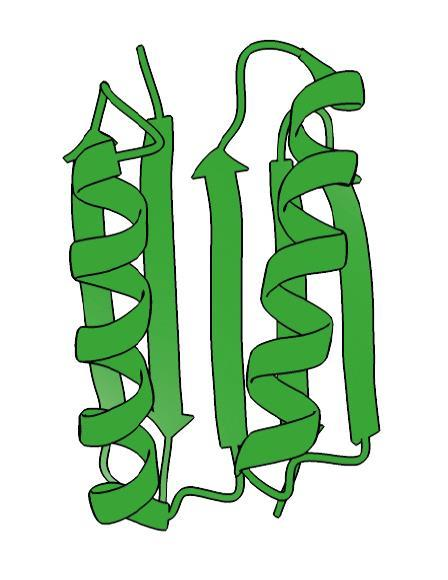
\includegraphics[height=5cm,keepaspectratio]{../../../theme/images/protein.png}
        };
      \end{tikzpicture}
      % Title
      \vspace*{0.5cm}
      \begin{center}
        {\Huge\color{iqbblue}\textbf{#2}}\\[0.3cm]
        {\Large\color{iqbgray}#1}
      \end{center}
      \vspace*{0.3cm}
    \endgroup
  \end{frame}
}

% 缩小子项缩进（本课程讲义使用更紧凑的层级）
\renewcommand{\subitem}[1]{%
  \par\vspace{2pt}%
  \noindent\hspace{0.8em}\textcolor{iqbblue}{$\circ$}\ #1%
}


% 设置教材信息
\iqbtextbook{Quantum Chemistry}{Levine}{7th Edition}{Pearson}

% 课程讲义元数据
\lecturetitle{第一章：薛定谔方程}
\lectureengtitle{Chapter 1: The Schrödinger Equation}

\author{东山月光下QM小组}
\date{\today}

\begin{document}

% ============================================================
% Footer Configuration
% ============================================================
\iqbfootline{default}{section}{pageofy}

% ------------------------------------------------------------
% 1. Cover
% ------------------------------------------------------------
\iqbcoverframe

% ------------------------------------------------------------
% 目录
% ------------------------------------------------------------
\begin{frame}{本章内容}
  \iqblayouttwo{
    \iqbsectiontitle{基本概念}
    \begin{iqbitemize}
    \item \textbf{1.1 量子化学简介}（Introduction to Quantum Chemistry）
      \item \textbf{1.2 历史背景}（Historical Background）
      \item \textbf{1.3 不确定性原理}（Uncertainty Principle）
      \item \textbf{1.4 含时薛定谔方程}（Time-Dependent Schrödinger Equation）
      \item \textbf{1.5 定态薛定谔方程}（Time-Independent Schrödinger Equation）
    \end{iqbitemize}
  }{
    \iqbsectiontitle{数学工具}
    \begin{iqbitemize}
    \item \textbf{1.6 概率论基础}（Probability Theory）
      \item \textbf{1.7 复数}（Complex Numbers）
      \item \textbf{1.8 SI单位制}（SI Units）
      \item \textbf{1.9 微积分公式}（Calculus Formulas）
    \end{iqbitemize}
  }
\end{frame}

% ============================================================
% Part 1: Quantum Chemistry (1.1)
% ============================================================
\iqbsectionframe{Quantum Chemistry}{量子化学}

% ------------------------------------------------------------
% 1.1-1. What is Quantum Chemistry
% ------------------------------------------------------------
\begin{frame}{量子化学：微观世界的定量描述}
  \iqblayouttwo{
    \iqbsectiontitle{经典力学的局限}
    \begin{iqbitemize}
    \item \textbf{17世纪末}：牛顿建立经典力学，成功描述宏观物体运动
      \item \textbf{20世纪初}：发现经典力学\textbf{无法正确}描述电子、原子核等\textbf{微观粒子}的行为
      \item 需要全新的理论框架（new theoretical framework）：\textbf{量子力学}

    \end{iqbitemize}
    \iqbsep

    \iqbsectiontitle{量子化学的定义}
    \begin{iqbitemize}
    \item 将\textbf{量子力学}应用于\textbf{化学问题}
      \item 微观粒子遵循量子力学定律（follow quantum laws）
      \item 利用量子力学原理理解和预测化学现象
      \item 结合统计力学（statistical mechanics）计算宏观热力学性质
    \end{iqbitemize}
  }{
    \iqbsectiontitle{量子效应的特征}
    \begin{iqbitemize}
    \item \textbf{能量量子化}（energy quantization）：能量只能取离散值
      \item \textbf{波粒二象性}（wave-particle duality）：粒子同时具有波动和粒子性质
      \item \textbf{不确定性}（uncertainty）：位置和动量不能同时精确测量
      \item \textbf{概率诠释}（probability interpretation）：只能预测概率而非确定结果
      \item \textbf{测量的影响}（measurement disturbance）：测量过程会改变系统状态

    \end{iqbitemize}
    \iqbsep

    \iqborangebox{核心思想}{量子力学用\textbf{波函数$\Psi$}描述微观粒子状态，用\textbf{薛定谔方程}描述其演化}
  }
\end{frame}

% ------------------------------------------------------------
% 1.1-2. Applications in Physical Chemistry
% ------------------------------------------------------------
\begin{frame}{量子化学在物理化学中的应用}
  \iqbfontsizemode{small}

  \iqblayouttwo{
    \iqbsectiontitle{热力学性质计算}
    \begin{iqbitemize}
    \item 利用统计力学，从量子力学能级计算宏观热力学量：
      \subitem{熵、热容、自由能}
      \subitem{适用于气体分子}
    \end{iqbitemize}
    \iqbsmallsep

    \iqbsectiontitle{分子光谱解释}
    \begin{iqbitemize}
    \item 解释分子光谱（molecular spectra）的频率和强度
      \item 通过光谱实验测定分子几何和性质：
        \subitem{分子几何结构}
          \subitem{偶极矩}
          \subitem{内旋转势垒}
          \subitem{构象异构体能量差}
    \end{iqbitemize}
    \iqbsmallsep

    \iqbsectiontitle{分子间相互作用}
    \begin{iqbitemize}
    \item 理解分子间作用力：范德华力、氢键等
      \item 预测晶体结构
      \item 理解固体中的化学键
    \end{iqbitemize}
  }{
    \iqbsectiontitle{分子性质理论计算}
    \begin{iqbitemize}
    \item 第一性原理（ab initio）计算分子性质
      \item 键长（bond length）、键角（bond angle）、键能（bond energy）
      \item 电子结构（electronic structure）与化学键（chemical bond）
      \item 激发态（excited state）与光化学性质（photochemical properties）

    \end{iqbitemize}
    \iqbsmallsep

    \iqbsectiontitle{化学反应动力学}
    \begin{iqbitemize}
    \item 计算过渡态（transition state）性质
      \item 估算反应速率常数（reaction rate constant）
      \item 深入理解反应机理（reaction mechanism）
      \item 预测反应选择性（reaction selectivity）

    \end{iqbitemize}
  }
\end{frame}

% ------------------------------------------------------------
% 1.1-3. Applications in Other Branches
% ------------------------------------------------------------
\begin{frame}{量子化学在其他化学分支的应用}
  \iqbfontsizemode{small}

  \iqblayouttwo{
    \iqbsectiontitle{有机化学}
    \begin{iqbitemize}
    \item 估算分子稳定性、计算反应中间体性质、研究反应机理（reaction mechanism）
    \item 分析和预测\textbf{NMR谱}，设计新型有机分子（novel organic molecules）
    \end{iqbitemize}
    \iqbsmallsep

    \iqbsectiontitle{分析化学}
    \begin{iqbitemize}
    \item 广泛使用各种光谱方法（spectroscopic methods）：UV-Vis、IR、Raman、NMR等
    \item 光谱的频率和强度\textbf{只能}通过量子力学正确理解和解释
    \end{iqbitemize}
    \iqbsmallsep

    \iqbsectiontitle{无机化学}
    \begin{iqbitemize}
    \item \textbf{配体场理论}（ligand field theory）：使用近似量子力学方法
    \item 准确预测过渡金属配合物的d轨道分裂（d-orbital splitting）、光谱（spectra）和磁性（magnetism）
    \end{iqbitemize}
  }{
    \iqbsectiontitle{生物化学}
    \begin{iqbitemize}
    \item 量子化学研究应用于生物分子构象、酶-底物结合、生物分子的溶剂化
    \item 酶催化反应机理研究（QM/MM方法）
    \end{iqbitemize}
    \iqbsmallsep

    \iqbsectiontitle{纳米材料}
    \begin{iqbitemize}
    \item \textbf{纳米材料}（1-100 nm）：量子力学决定其特殊光学和电子性质
    \item 尺寸<100 nm时，光学、电子、化学性质与体相材料（bulk materials）显著不同
    \item 量子阱（quantum well）、量子线（quantum wire）、量子点（quantum dot）
    \end{iqbitemize}
  }
\end{frame}

% ------------------------------------------------------------
% 1.1-4. Modern Computational Chemistry
% ------------------------------------------------------------
\begin{frame}{现代计算化学的发展}
  \iqbfontsizemode{small}

  \iqblayouttwo{
    \iqbsectiontitle{计算能力与软件}
    \begin{iqbitemize}
    \item 计算机处理速度的快速增长（rapid growth）
    \item 新方法使量子化学成为实用工具：\textbf{密度泛函理论}（DFT）、多体微扰理论、耦合簇理论
    \item 商业化软件：Gaussian、ORCA、Molpro等，设计给\textbf{所有化学家}使用
    \item 用户友好的图形界面（user-friendly graphical interface）降低了使用门槛
    \end{iqbitemize}
    \iqbsmallsep

    \iqbsectiontitle{新期刊的创立}
    \begin{iqbitemize}
    \item 美国化学会2005年创办新期刊：
      \subitem{\textit{Journal of Chemical Theory and Computation}}
      \subitem{专注理论和计算化学的期刊（theoretical and computational chemistry）}
    \end{iqbitemize}
  }{
    \iqbsectiontitle{量子力学的重要性}
    \begin{iqbitemize}
    \item Stephen Hawking (1988)：
      \subitem{\textit{"量子力学……是几乎所有现代科学和技术的基础"}}
      \subitem{\textit{"它控制晶体管和集成电路的行为"}}
      \subitem{\textit{"是现代化学和生物学的基础"}}
    \item 量子力学决定纳米材料性质：量子阱、量子线、量子点
    \item 与体相材料性质显著不同
    \end{iqbitemize}
    \iqbsmallsep

    \iqbsectiontitle{实际应用}
    \begin{iqbitemize}
    \item 药物设计（drug design）：计算机辅助药物分子设计
    \item 材料科学：新型功能材料的预测和优化
    \item 催化机理：理解催化反应的微观机制
    \end{iqbitemize}
  }
\end{frame}

% ------------------------------------------------------------
% Part 2: Historical Background (1.2)
% ============================================================
\iqbsectionframe{Historical Background}{量子力学的历史背景}

% ------------------------------------------------------------
% 1.2-1. Light as a Wave
% ------------------------------------------------------------
\begin{frame}{光的波动本质：实验证据的建立}
  \iqbfontsizemode{small}
  \iqblayouttwo{
    \iqbsectiontitle{Young双缝实验（1803）}
    \begin{iqbitemize}
    \item Thomas Young通过双针孔实验观察到\textbf{衍射}和\textbf{干涉}现象
      \subitem{\textbf{衍射}（diffraction）：波绕过障碍物发生弯曲}
      \subitem{\textbf{干涉}（interference）：两列同频率波叠加}
      \subitem{每点的扰动 = 各波扰动的矢量和}
    \item 提供了光的波动性的令人信服的证据
    \end{iqbitemize}
    \iqbsep

    \iqbsectiontitle{Maxwell电磁理论（1864）}
    \begin{iqbitemize}
    \item James Clerk Maxwell发表\textbf{Maxwell方程组}
      \subitem{统一了电学和磁学定律（unified electricity and magnetism）}
      \subitem{预言加速电荷会以\textbf{电磁波}形式辐射能量}
      \subitem{预测的波速 = 实验测得的光速}
    \item 结论：\textbf{光是一种电磁波}
    \end{iqbitemize}
  }{
    \iqbsectiontitle{Hertz实验验证（1888）}
    \begin{iqbitemize}
    \item Heinrich Hertz探测到火花中加速电荷产生的无线电波
      \subitem{完全符合Maxwell方程组的预言}
    \item 确认：光确实是电磁波
    \end{iqbitemize}
    \iqbsep

    \iqbsectiontitle{电磁波的基本关系}
    \begin{iqbitemize}
    \item 真空中所有电磁波速度：$c = 2.998 \times 10^8$ m/s
      \subitem{频率$\nu$与波长$\lambda$的关系：}
    \end{iqbitemize}
      \[
        \lambda \nu = c
      \]
    \begin{iqbitemize}
  \item 按频率递增：无线电波、微波、红外、可见光、紫外、X射线、$\gamma$射线
  \item 波长单位：1 nm = $10^{-9}$ m，1 \AA\ = $10^{-10}$ m = 0.1 nm
    \end{iqbitemize}
  }
\end{frame}

% ------------------------------------------------------------
% 1.2-2. Blackbody Radiation - Problem
% ------------------------------------------------------------
\begin{frame}{黑体辐射问题：经典物理学的困境}
  \iqbfontsizemode{small}

  \iqblayouttwo{
    \iqbsectiontitle{黑体辐射实验（1890s）}
    \begin{iqbitemize}
    \item 黑体（blackbody）：吸收所有入射光的物体
      \item 近似实现：带小孔的空腔（cavity with tiny hole）
      \item 测量：不同温度下，不同频率光的辐射强度
      \item 实验结果：黑体辐射强度分布随温度变化

    \end{iqbitemize}
    \iqbsmallsep

    \iqbsectiontitle{Wien公式（1896）}
    \begin{iqbitemize}
    \item Wien提出黑体辐射的经验公式（empirical formula）：
    \end{iqbitemize}
      \[
        I = a\nu^3 e^{-b\nu/T}
      \]
    \begin{iqbitemize}
      \item $I \mathrm{d}\nu$：频率在$\nu$到$\nu+\mathrm{d}\nu$范围内，单位时间单位面积辐射的能量
      \item 与1896年的实验数据吻合良好
      \item 但理论推导不被物理学家接受
    \end{iqbitemize}
  }{
    \iqbsectiontitle{低频数据的偏离（1899-1900）}
    \begin{iqbitemize}
    \item 测量范围扩展到更低频率（lower frequencies）
      \item 低频数据与Wien公式有显著偏差
      \item 经典物理理论无法解释实验结果（classical physics failed）

    \end{iqbitemize}
    \iqbsmallsep

    \iqbsectiontitle{Planck公式（1900年10月）}
    \begin{iqbitemize}
    \item Max Planck提出新公式：
    \end{iqbitemize}
      \[
        I = \dfrac{a\nu^3}{e^{b\nu/T} - 1}
      \]
    \begin{iqbitemize}
      \item 与\textbf{所有}频率的数据完美吻合
      \item 但需要理论推导来解释公式（theoretical derivation needed）

    \end{iqbitemize}
    \iqbsmallsep

    \iqborangebox{经典困境}{经典物理学无法解释黑体辐射的频率分布}
  }
\end{frame}

% ------------------------------------------------------------
% 1.2-3. Planck's Quantum Hypothesis
% ------------------------------------------------------------
\begin{frame}{Planck的量子假设：能量量子化}
  \iqbfontsizemode{small}

  \iqblayouttwo{
    \iqbsectiontitle{Planck的理论推导（1900年12月）}
    \begin{iqbitemize}
    \item 假设：黑体中的辐射发射体和吸收体是\textbf{谐振子}（harmonic oscillators）
      \item 频率为$\nu$的谐振子的总能量由$N$个不可分割的"能量元"组成
  \item 每个能量元的大小：$h\nu$ $N$是整数，$h$是新的物理常数（\textbf{Planck常数}）
      \item 效果：限制每个谐振子的能量为$h\nu$的整数倍
      \item 即：\textbf{能量量子化}

    \end{iqbitemize}
    \iqbsmallsep

    \iqbsectiontitle{理论结果}
    \begin{iqbitemize}
  \item 推导出：$a = 2\pi h/c^2$，$b = h/k$ $k$：Boltzmann常数
      \item 通过拟合黑体辐射实验曲线确定：$h = 6.6 \times 10^{-34}$ J·s
    \end{iqbitemize}
    
  \iqbgreenbox{量子概念}{能量只能以离散值（量子）存在，不能连续变化}
  }{
    \iqbsectiontitle{量子力学的诞生}
    \begin{iqbitemize}
    \item Planck的工作通常被认为是\textbf{量子力学的开端}
      \item 但历史学家争论：Planck在1900年是否真的认为能量量子化是物理实在
      \item 还是仅仅是数学近似而非物理现实（mathematical approximation）？

    \end{iqbitemize}
    \iqbsmallsep

    \iqbsectiontitle{革命性意义}
    \begin{iqbitemize}
    \item \textbf{能量量子化}能量量子化与之前的物理学思想直接矛盾（contradicted classical physics）
      \item 根据牛顿力学，物质物体的能量可以\textbf{连续变化}
      \item 但只有量子化能量假设才能得到正确的黑体辐射曲线
  \item Kragh：\textit{"如果1900年12月物理学发生了革命，似乎没人注意到。Planck也不例外"} 重要性是事后的历史重构
    \end{iqbitemize}
  }

\end{frame}

% ------------------------------------------------------------
% 1.2-4. Photoelectric Effect
% ------------------------------------------------------------
\begin{frame}{光电效应：光的粒子性}
  \iqbfontsizemode{small}

  \iqblayouttwo{
    \iqbsectiontitle{光电效应现象}
    \begin{iqbitemize}
    \item \textbf{光电效应}（photoelectric effect）：光照射金属表面 $\rightarrow$ 发射电子
        \subitem{波的能量$\propto$强度，与频率无关}
          \subitem{预期：光电子动能随光强增加而增加}
          \subitem{预期：光电子动能与频率无关}
    \item \textbf{实际观察}：经典电磁波理论无法解释
        \subitem{光电子动能与光强\textbf{无关}}
          \subitem{光电子动能随频率\textbf{增加}而增加}

    \end{iqbitemize}
    \iqbsmallsep

    \iqbsectiontitle{Einstein的解释（1905）}
    \begin{iqbitemize}
    \item 光由类粒子实体组成：\textbf{光子}（photons）
      \item 光子模型中每个光子能量（photon energy）：
    \end{iqbitemize}
      \[
        E_{\text{photon}} = h\nu
      \]
    \begin{iqbitemize}
      \item 金属中的电子吸收一个光子（electron absorbs photon）
    \end{iqbitemize}
  }{
    \iqbsectiontitle{根据能量守恒定律关系：}
    \begin{iqbitemize}
    \item 光子能量部分用于克服金属的束缚
      \item 光子能量其余部分转化为电子动能（converted to kinetic energy）
      \item 根据根据能量守恒定律（energy conservation law）定律（energy conservation）：
    \end{iqbitemize}
      \[
        h\nu = \Phi + T
      \]
    \begin{iqbitemize}
      \item $\Phi$：\textbf{功函数}（work function），电子逃逸所需最小能量
      \item $T$光电子的最大动能（maximum kinetic energy）：
      \item 增加光频率$\nu$ $\rightarrow$ 增加光子能量 $\rightarrow$ 增加电子动能
      \item 增加光强（固定频率）$\rightarrow$ 增加光子数 $\rightarrow$ 增加电子发射率，但不改变单个电子动能

    \end{iqbitemize}
    \iqbtinysep

    \iqbgreenbox{波粒二象性}{光既表现出\textbf{波动性}（diffraction、interference），也表现出\textbf{粒子性}（photoelectric effect）}
  }
\end{frame}

% ------------------------------------------------------------
% 1.2-5. Atomic Structure - Rutherford Scattering
% ------------------------------------------------------------
\begin{frame}{原子结构的探索：Rutherford散射实验}
  \iqbfontsizemode{small}

  \iqblayouttwo{
    \iqbsectiontitle{19世纪末的发现}
    \begin{iqbitemize}
    \item 放电管和放射性研究表明 原子由\textbf{带电粒子}组成
      \item \textbf{电子}（electron）：带负电（negative charge）
      \item \textbf{质子}：带正电，质量为电子1836倍
      \item 电子和质子电量相等，符号相反（equal magnitude, opposite sign）
      \item \textbf{中子}（neutron）：不带电（discovered in 1932）

    \end{iqbitemize}
    \iqbtinysep

    \iqbsectiontitle{Rutherford散射（1909-1911）}
    \begin{iqbitemize}
    \item Rutherford、Geiger、Marsden
      \item $\alpha$粒子束穿过薄金属箔
      \item 用荧光屏观察粒子偏转
      \item 结果：
        \subitem{大多数几乎\textbf{不偏转}}
          \subitem{少数\textbf{大角度偏转}}
          \subitem{个别\textbf{反向散射}}
    \end{iqbitemize}
  }{
    \iqbsectiontitle{理论分析}
    \begin{iqbitemize}
    \item 大偏转需电荷很近 $\rightarrow$ 库仑斥力大
      \item J.J. Thomson模型（1904）：
        \subitem{正电荷分布于整个原子}
          \subitem{中心斥力为零，\textbf{无法解释}大角散射}
      \item Rutherford实验结论（Rutherford's conclusion）：
        \subitem{正电荷集中在\textbf{微小重核}中}
          \subitem{才能产生大散射角}

    \end{iqbitemize}
    \iqbtinysep

    \iqbsectiontitle{原子的结构}
    \begin{iqbitemize}
    \item 原子含微小($10^{-13}$--$10^{-12}$ cm)、重的\textbf{原子核}（nucleus）
      \item 核由中子和$Z$个质子组成，核外有$Z$个电子
      \item 带电粒子通过库仑定律（Coulomb's law）相互作用
      \item 原子半径 $\approx$ 1 Å
      \item 分子由多个原子核和电子组成（molecules have multiple nuclei）
    \end{iqbitemize}
  }
\end{frame}

% ------------------------------------------------------------
% 1.2-6. Bohr Model
% ------------------------------------------------------------
\begin{frame}{Bohr原子模型：量子化轨道}
  \iqbfontsizemode{small}

  \iqblayouttwo{
    \iqbsectiontitle{Rutherford行星模型的困难（1911）}
    \begin{iqbitemize}
    \item Rutherford提出：电子绕核运动，类似行星绕太阳
  \item 但有根本困难 根据经典电磁理论：
        \subitem{加速运动的带电粒子会辐射电磁波}
          \subitem{圆周运动中速度方向不断变化 $\rightarrow$ 有加速度}
          \subitem{电子应不断辐射能量}
          \subitem{电子应螺旋坠入原子核}
      \item 因此，按经典物理：Rutherford原子\textbf{不稳定}，会\textbf{坍塌}

    \end{iqbitemize}
    \iqbsmallsep

    \iqbsectiontitle{Bohr的量子化假设（1913）}
    \begin{iqbitemize}
    \item Bohr将\textbf{能量量子化}应用于氢原子
      \item 核心假设：电子轨道能量量子化（electron energy quantization）
      \item 电子只能在若干\textbf{定态轨道}（stationary orbits）上运动
      \item 电子在允许轨道上运动时不辐射能量（no radiation in allowed orbits）\textbf{不辐射}
    \end{iqbitemize}
  }{
    \iqbsectiontitle{光谱公式}
    \begin{iqbitemize}
    \item 电子在轨道间跃迁时吸收或发射光子
      \item 光子频率$\nu$满足：
    \end{iqbitemize}
      \[
        E_{\text{upper}} - E_{\text{lower}} = h\nu
      \]
    \begin{iqbitemize}
      \item 根据能量守恒定律（energy conservation law）
      \subitem{使用经典力学推导氢原子能级公式}
      \subitem{用式(1.4)计算，与观察到的氢光谱一致}

    \end{iqbitemize}
    \iqbsmallsep

    \iqbsectiontitle{Bohr模型的局限}
    \begin{iqbitemize}
    \item Bohr模型无法拟合氦原子光谱（failed for helium spectrum）
      \item 无法解释分子中的化学键形成（chemical bonding）
      \item 失败原因：用\textbf{经典力学}描述电子运动
      \item 原子光谱显示离散频率 $\rightarrow$ 能量量子化
      \item 但经典力学允许能量连续变化（classical: continuous energy），矛盾！
    \end{iqbitemize}
  }
\end{frame}

% ------------------------------------------------------------
% 1.2-7. de Broglie Wave-Particle Duality
% ------------------------------------------------------------
\begin{frame}{de Broglie物质波：波动性的普遍性}
  \iqbfontsizemode{small}

  \iqblayoutcustom[0.48]{
    \iqbsectiontitle{历史背景与假设（1923）}
    \begin{iqbitemize}
    \item \textbf{原子光谱}：离散频率表明电子能量\textbf{量子化}
    \item \textbf{波动类比}：提琴弦的基频和泛音同样显示量子化
    \item de Broglie（1923）：电子运动有\textbf{波动}aspect
    \end{iqbitemize}
      \[
        \boxed{\lambda = \dfrac{h}{mv} = \dfrac{h}{p}}
      \]
    \begin{iqbitemize}
    \item \textbf{推理过程}：类比光子
    \item 光子能量：$E = pc$（相对论）+ $E = h\nu = hc/\lambda$
    \item 推导：$pc = hc/\lambda \Rightarrow \lambda = h/p$（光子）
    \item 推广到电子：$\lambda = h/p$（物质波公式）
    \end{iqbitemize}
    \iqbtinysep

    \iqbsectiontitle{实验验证：从电子到大分子}
    \begin{iqbitemize}
    \item \textbf{1927}：Davisson-Germer实验（电子衍射）
    \item \textbf{1932}：Stern观察He、H$_2$同样效应
    \item \textbf{现代验证}：C$_{60}$富勒烯、C$_{48}$H$_{26}$F$_{24}$N$_8$O$_8$大分子衍射
    \item 实验证明波动性是微观粒子的内禀性质（\textit{intrinsic wave nature}）
    \end{iqbitemize}
  }{
    \centering
    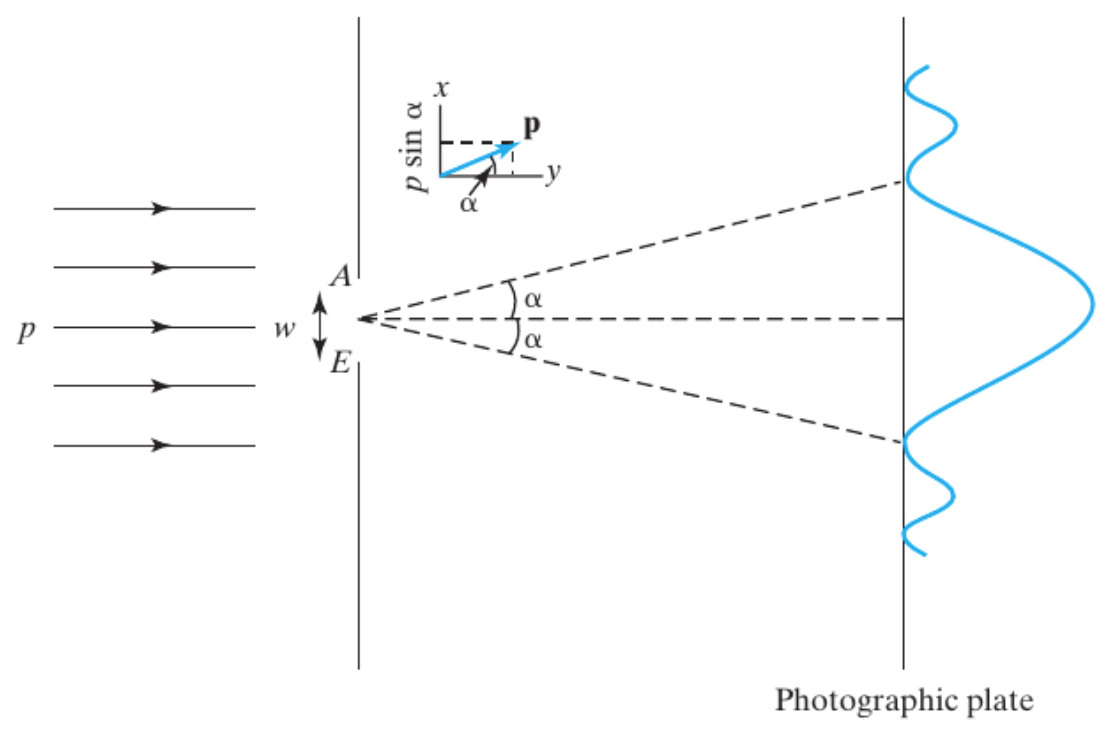
\includegraphics[height=0.45\textheight]{Figures/fig1_1_diffraction.png}

    \iqbmicrosep

    {\scriptsize 图1.1：电子衍射图样证明电子波动性。从电子到C$_{60}$等大分子，衍射实验验证了波动性的普遍性。}
  }
\end{frame}

% ------------------------------------------------------------
% 1.2-8. Human Understanding Limitation
% ------------------------------------------------------------
\begin{frame}{微观世界：超越人类直觉}
  \iqbfontsizemode{small}

  \iqblayouttwo{
    \iqbsectiontitle{为什么理解困难？}
    \begin{iqbitemize}
    \item 经典概念来自\textbf{宏观}经验，不能描述\textbf{微观}
      \item 人脑进化处理宏观现象，\textbf{未被设计}处理原子、分子现象
      \item 人类无法完全理解但也必须接受（must accept counterintuitive reality）\textbf{不足为奇}

    \end{iqbitemize}
    \iqbtinysep

    \iqbsectiontitle{光子vs电子}
    \begin{iqbitemize}
    \item 都有二象性，但\textbf{不同}实体
      \item \textbf{光子}：速度$c$，静质量0，用相对论
      \item \textbf{电子}：$v < c$，非零质量，慢时用非相对论
    \end{iqbitemize}
  }{
    \iqbsectiontitle{需要新的理论}
    \begin{iqbitemize}
    \item 经典力学在微观尺度完全失败（classical mechanics fails at micro scale）
      \item 需要\textbf{量子力学}，用\textbf{波函数$\Psi$}描述粒子
      \item 用\textbf{薛定谔方程}描述演化
      \item 概率诠释（probability interpretation）取代经典确定性（replaces determinism）

    \end{iqbitemize}
    \iqbtinysep

    \iqbsectiontitle{哲学启示}
    \begin{iqbitemize}
    \item 人类理解受限于宏观进化经验（intuition shaped by macroscopic experience）
      \item 微观粒子行为超越日常直觉（beyond everyday intuition）
      \item 需接受新的概念框架
    \end{iqbitemize}
  }
\end{frame}

% ------------------------------------------------------------
% Example: de Broglie Wavelength Calculation
% ------------------------------------------------------------
\begin{frame}{例题：de Broglie波长计算}
  \iqbfontsizemode{small}

  \iqblayouttwo{
    \iqbsectiontitle{题目（Problem 1.6）}
    \begin{iqbitemize}
    \item 计算以光速1/137运动的电子的de Broglie波长
      \item 已知：$c = 2.998 \times 10^8$ m/s，
    \end{iqbitemize}
          $m_e = 9.109 \times 10^{-31}$ kg，
          $h = 6.626 \times 10^{-34}$ J·s

    \iqbtinysep

    \iqbsectiontitle{解题思路}
    \begin{iqbitemize}
    \item 使用de Broglie关系：$\lambda = h/(mv)$
      \item 先算速度$v$，再算动量$p$，最后算波长
    \end{iqbitemize}
  }{
    \iqbsectiontitle{详细计算}
    \begin{iqbitemize}
    \item 速度：
    \end{iqbitemize}
      \[
        v = c/137 = 2.188 \times 10^6 \text{ m/s}
      \]
    \begin{iqbitemize}
      \item 动量：
    \end{iqbitemize}
      \[
        p = m_e v = 1.993 \times 10^{-24} \text{ kg·m/s}
      \]
    \begin{iqbitemize}
      \item 波长：
    \end{iqbitemize}
      \[
        \lambda = h/p = 3.324 \times 10^{-10} \text{ m}
      \]
      \[
        \boxed{\lambda = 3.324 \text{ Å} = 0.3324 \text{ nm}}
      \]

    \iqbtinysep

    \iqbsectiontitle{物理意义}
    \begin{iqbitemize}
    \item 波长约为原子尺度（$\sim$0.1 nm量级）
      \item 解释电子衍射实验观察到的衍射图样
      \item 证明物质波是可观测的物理现象
    \end{iqbitemize}
  }
\end{frame}

% ============================================================
% Part 3: Uncertainty Principle (1.3)
% ============================================================
\iqbsectionframe{Uncertainty Principle}{不确定性原理}

% ------------------------------------------------------------
% 1.3-1. Single-Slit Diffraction Experiment
% ------------------------------------------------------------
\begin{frame}{单缝衍射实验：实验装置与现象}
  \iqbfontsizemode{small}

  \iqblayoutcustom[0.50]{
    \iqbsectiontitle{实验装置与现象}
    \begin{iqbitemize}
    \item 一束准直的电子束射向宽度为$w$的狭缝
      \item 缝后放置感光板或探测器记录电子位置
      \item 观察到明显的\textbf{衍射图样}（diffraction pattern）而非简单的几何投影
      \item 图样特点：中央亮纹最宽最亮，两侧对称分布暗纹和次级亮纹
      \item 这是电子具有\textbf{波动性}的直接实验证据

    \end{iqbitemize}
    \iqbtinysep

    \iqbsectiontitle{衍射图样的物理意义}
    \begin{iqbitemize}
    \item 衍射说明电子通过狭缝后动量方向发生改变
      \item 部分动量转移到横向方向，产生$x$方向的动量分量$p_x$
      \item 中央最大值对应大部分电子到达的位置
      \item 衍射图样的宽度与狭缝宽度$w$和德布罗意波长$\lambda$相关
      \item 衍射现象无法用经典粒子运动轨迹解释

    \end{iqbitemize}
  }{
    \centering
    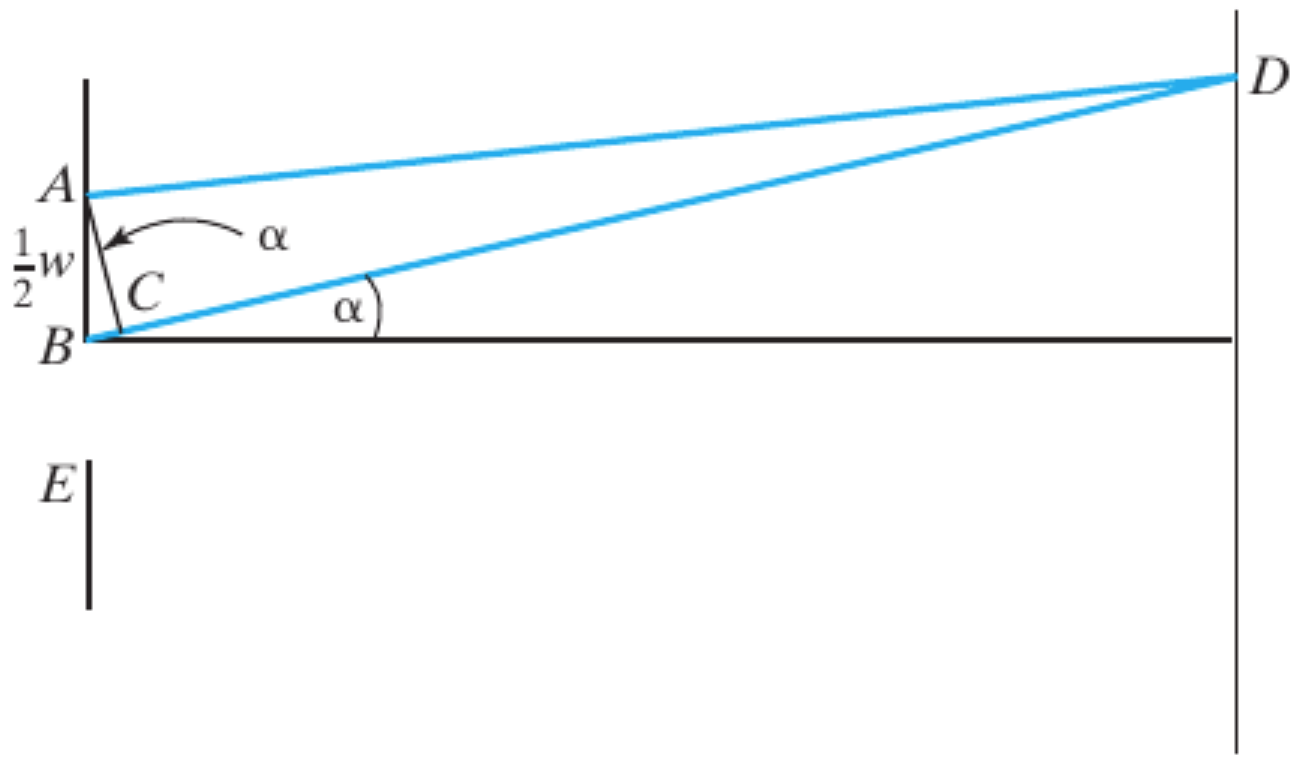
\includegraphics[height=0.48\textheight]{Figures/fig1_2_calculation.png}

    \iqbmicrosep

    {\scriptsize 图1.2：单缝衍射实验示意}
  }
\end{frame}

\begin{frame}{单缝衍射实验：定量分析与意义}
  \iqbfontsizemode{small}

  \iqblayouttwo{
    \iqbsectiontitle{衍射图样定量分析}
    \begin{iqbitemize}
  \item 第一暗纹位置满足条件：$\sin\theta_1 = \lambda/w$ 其中$\theta_1$是从中心到第一暗纹的角度
      \item 大部分电子落在中央亮纹（$-\theta_1$到$+\theta_1$范围内）
  \item 小角度近似：当$\theta_1$很小时，$\sin\theta_1 \approx \theta_1 \approx \lambda/w$ 狭缝越窄，衍射越明显，中央亮纹越宽
    \end{iqbitemize}
    \iqbtinysep

    \iqborangebox{核心洞察}{衍射现象意味着：限制粒子在空间中的位置会不可避免地改变其动量分布}
  }{
    \iqbsectiontitle{波动性与粒子性}
    \begin{iqbitemize}
    \item \textbf{粒子性}：电子作为离散的粒子被探测到
      \item \textbf{波动性}：电子束产生衍射和干涉图样
      \item 单个电子重复实验也会产生相同衍射图样
      \item 说明波粒二象性是微观粒子的基本属性
      \item 衍射实验是理解不确定关系的关键
    \end{iqbitemize}
    \iqbtinysep

    \iqbgreenbox{关键结论}{电子的位置测量（通过狭缝）和动量分布（通过衍射图样）相互关联}
  }
\end{frame}

% ------------------------------------------------------------
% 1.3-2. Derivation of Uncertainty Relation
% ------------------------------------------------------------
\begin{frame}{不确定性关系的推导（1/2）}
  \iqbfontsizemode{small}

  \iqblayouttwo{
    \iqbsectiontitle{位置不确定度}
    \begin{iqbitemize}
    \item 电子通过狭缝时，位置测量受缝宽$w$限制（position uncertainty）
      \item $x$坐标的不确定度（uncertainty）：
    \end{iqbitemize}
      \[
        \Delta x \approx w
      \]
    \begin{iqbitemize}
      \item 狭缝越窄，位置测量越精确，但衍射效应越强
    \end{iqbitemize}
    \iqbtinysep

    \iqbsectiontitle{动量不确定度}
    \begin{iqbitemize}
    \item 通过狭缝后，电子形成衍射图样（diffraction pattern）
      \item 说明电子获得了$x$方向的动量分量$p_x$
      \item 大部分电子落在中央亮纹内（角度$-\theta$到$+\theta$）
      \item 动量不确定度约为：
    \end{iqbitemize}
      \[
        \Delta p_x \approx 2p\sin\theta \approx 2p\theta
      \]
  }{
    \iqbsectiontitle{数学推导}
    \begin{iqbitemize}
    \item \textbf{第一步}：单缝衍射第一暗纹条件（first dark fringe）：
    \end{iqbitemize}
      \[
        \sin\theta \approx \theta \approx \dfrac{\lambda}{w}
      \]
    \begin{iqbitemize}
      \item \textbf{第二步}：代入动量不确定度：
    \end{iqbitemize}
      \[
        \Delta p_x \approx 2p\dfrac{\lambda}{w}
      \]
    \begin{iqbitemize}
      \item \textbf{第三步}：利用德布罗意关系$\lambda = h/p$（de Broglie relation）：
    \end{iqbitemize}
      \[
        \Delta p_x \approx \dfrac{2h}{w}
      \]
    \begin{iqbitemize}
      \item \textbf{第四步}：代入$\Delta x \approx w$：
    \end{iqbitemize}
      \[
        \Delta x \cdot \Delta p_x \approx w \cdot \dfrac{2h}{w} \approx 2h
      \]
    \begin{iqbitemize}
    \item \textbf{结论}：位置和动量的不确定度乘积为有限值（finite product）
    \end{iqbitemize}
    \iqbtinysep
  }
\end{frame}

\begin{frame}{不确定性关系的推导（2/2）}
  \iqbfontsizemode{small}

  \begin{iqbitemize}
  \item \textbf{第四步}：代入位置不确定度$\Delta x \approx w$
  \end{iqbitemize}
    \[
      \Delta x \cdot \Delta p_x \approx w \cdot \dfrac{2h}{w} \approx 2h
    \]
  \begin{iqbitemize}
  \item \textbf{结论}：位置和动量的不确定度乘积为有限值
  \end{iqbitemize}

  \iqbsectiontitle{结果讨论}
  \begin{iqbitemize}
  \item 这是粗略估计，严格量子力学推导给出精确结果
    \item 海森堡于1927年提出不确定性原理
  \item 量子力学严格证明得到：$\Delta x \cdot \Delta p_x \geq \hbar/2$ $\hbar = h/(2\pi)$ 是约化Planck常数
    \item 不等式说明不确定度乘积有下限，不能无限小
  \end{iqbitemize}
\end{frame}

\begin{frame}{不确定性关系的物理意义}
  \iqbfontsizemode{small}

  \iqblayouttwo{
    \iqbsectiontitle{物理意义}
    \begin{iqbitemize}
    \item 无法同时精确测量位置和动量
      \item 测量精度受基本物理常数的限制
      \item 不是测量技术的缺陷，而是自然的本质
      \item 精确的位置测量必然导致动量的较大分散
      \item 这源于微观粒子的波粒二象性
    \end{iqbitemize}
    \iqbtinysep

    \iqbgreenbox{本质属性}{不确定性是量子系统的基本属性，而非测量不完善}
  }{
    \iqbsectiontitle{对经典物理的冲击}
    \begin{iqbitemize}
    \item \textbf{经典力学}：粒子有确定的轨迹和位置、动量
      \item \textbf{量子力学}：只能预测概率，位置和动量不能同时精确确定
      \item 这标志着物理学从决定论向概率论的转变
      \item 不仅是理论限制，实验已反复验证
      \item 对所有微观粒子普遍成立
    \end{iqbitemize}
    \iqbtinysep

    \iqborangebox{重要意义}{不确定性原理是区分经典物理和量子物理的核心概念之一}
  }
\end{frame}

% ------------------------------------------------------------
% 1.3-2b. Heisenberg Uncertainty Principle
% ------------------------------------------------------------
\begin{frame}{海森堡不确定性原理}
  \iqbfontsizemode{small}

  \iqblayouttwo{
    \iqbsectiontitle{不确定性原理的精确表述}
    \begin{iqbitemize}
    \item 海森堡于1927年提出，经严格量子力学推导得到：
    \end{iqbitemize}
      \[
        \boxed{\Delta x \cdot \Delta p_x \geq \dfrac{\hbar}{2}}
      \]
    \begin{iqbitemize}
      \item $\hbar = h/(2\pi) = 1.055 \times 10^{-34}$ J·s，读作"h-bar"
      \item $\hbar$称为约化Planck常数，是量子力学的基本常数
      \item 这是\textbf{自然的基本限制}，与测量技术无关
      \item 不等式说明位置和动量的不确定度乘积有下限
      \item 等号对应最小不确定度波包（高斯波包）
    \end{iqbitemize}
    \iqbtinysep

    \iqbsectiontitle{深刻物理意义}
    \begin{iqbitemize}
    \item 微观粒子的位置和动量\textbf{不能同时精确确定}
      \item 这不是因为测量设备不够精确或存在测量干扰
      \item 而是量子力学系统的\textbf{内在性质}和基本特征
      \item 粒子本身就不存在同时精确的位置和动量
      \item 经典力学中粒子运动轨迹的概念在量子层面失效
      \item 微观粒子不能用"位置随时间变化的轨道"描述
    \end{iqbitemize}
  }{
    \iqbsectiontitle{三维空间的不确定性关系}
    \begin{iqbitemize}
    \item 不确定性关系对三个坐标轴分别成立
  \item $\Delta x \cdot \Delta p_x \geq \hbar/2$，$\Delta y \cdot \Delta p_y \geq \hbar/2$，$\Delta z \cdot \Delta p_z \geq \hbar/2$ 不同方向的不确定性相互独立
      \item 例如：$x$方向位置精确不影响$y$方向动量的测量精度
    \end{iqbitemize}
    \iqbtinysep

    \iqbsectiontitle{其他共轭变量}
    \begin{iqbitemize}
    \item \textbf{能量-时间不确定性}（energy-time uncertainty）：$\Delta E \cdot \Delta t \geq \hbar/2$
      \item 能量测量需要时间，短时间测量能量不确定度大
      \item 所有\textbf{共轭变量}（conjugate variables）对都满足类似的不确定性关系
    \end{iqbitemize}
  }
\end{frame}

% ------------------------------------------------------------
% 1.3-3. Physical Meaning: Complementarity and Measurement
% ------------------------------------------------------------
\begin{frame}{不确定性原理的物理意义：互补性与测量}
  \iqbfontsizemode{small}

  \iqblayouttwo{
    \iqbsectiontitle{互补关系}
    \begin{iqbitemize}
    \item 位置测量越精确（$\Delta x$越小）
      \item 动量就越不确定（$\Delta p_x$越大）
      \item 反之亦然
      \item 这是\textbf{互补原理}（complementarity principle）的体现

    \end{iqbitemize}
    \iqbsep

    \iqbsectiontitle{对经典轨迹概念的否定}
    \begin{iqbitemize}
    \item 经典力学：粒子有确定的轨迹
      \item 每时刻都有确定的位置$x(t)$和动量$p(t)$
  \item 量子力学：\textbf{轨迹概念无意义} 不能同时精确知道$x$和$p$
      \item 就不能确定轨迹
      \item 只能用\textbf{波函数}$\Psi(x,t)$描述状态
    \end{iqbitemize}
  }{
    \iqbsectiontitle{测量的影响}
    \begin{iqbitemize}
    \item 测量位置：使用光子照射电子
      \item 光子与电子碰撞 $\rightarrow$ 改变电子动量
      \item 精确测量位置 $\rightarrow$ 需要短波长光子（高能量）
      \item 高能量光子 $\rightarrow$ 对动量扰动大
      \item 测量行为\textbf{不可避免}地影响系统

    \end{iqbitemize}
    \iqbsep

    \iqbsectiontitle{量子测量的本质}
    \begin{iqbitemize}
    \item 测量不仅仅是"观察"
      \item 而是\textbf{与系统相互作用}
      \item 这种相互作用改变系统状态
      \item 不确定性是\textbf{自然规律}，非技术限制
    \end{iqbitemize}
  }

  \iqbgreenbox{核心洞察}{测量行为本质上改变系统，量子世界的不确定性是内在的}
\end{frame}

% ------------------------------------------------------------
% 1.3-3b. Macroscopic vs Microscopic Scale
% ------------------------------------------------------------
\begin{frame}{不确定性原理：宏观与微观的对比}
  \iqblayouttwo{
    \iqbsectiontitle{为何日常生活感受不到？}
    \begin{iqbitemize}
    \item $\hbar$非常小：$1.055 \times 10^{-34}$ J·s
      \item 对宏观物体（$m \sim$ g级）：
        \subitem{$\Delta x \cdot \Delta p_x \geq \hbar/2 \approx 10^{-34}$ J·s}
          \subitem{典型$\Delta p_x \sim 10^{-5}$ kg·m/s}
          \subitem{$\Rightarrow$ $\Delta x \sim 10^{-29}$ m}
          \subitem{远小于任何可测尺度，可忽略}
      \item 宏观世界\textbf{近似}为经典力学
    \end{iqbitemize}
  }{
    \iqbsectiontitle{微观粒子的量子效应}
    \begin{iqbitemize}
    \item 对微观粒子（原子中电子）：
        \subitem{$\Delta x \sim 10^{-10}$ m（原子尺度）}
          \subitem{$\Rightarrow$ $\Delta p_x \geq \hbar/(2\Delta x) \sim 10^{-24}$ kg·m/s}
          \subitem{电子质量$m_e = 9.1 \times 10^{-31}$ kg}
          \subitem{$\Rightarrow$ $\Delta v_x \geq 10^6$ m/s}
          \subitem{与电子速度同量级！}
      \item 不确定性\textbf{主导}微观行为
    \end{iqbitemize}
  }

  \iqborangebox{尺度效应}{不确定性原理对微观粒子至关重要，对宏观物体可忽略}

  \iqbgreenbox{哲学含义}{自然在基本层面上是\textbf{内在随机}的，决定论在量子层面不成立}
\end{frame}

% ============================================================
% Part 4: Time-Dependent Schrödinger Equation (1.4)
% ============================================================
\iqbsectionframe{Time-Dependent Schrödinger Equation}{含时薛定谔方程}

% ------------------------------------------------------------
% 1.4-1. Classical Mechanics Review
% ------------------------------------------------------------
\begin{frame}{经典力学回顾：牛顿第二定律}
  \iqbfontsizemode{small}

  \iqblayouttwo{
    \iqbsectiontitle{牛顿运动定律}
    \begin{iqbitemize}
    \item 经典力学基本方程：
    \end{iqbitemize}
      \[
        \boxed{F = ma = m\dfrac{d^2x}{dt^2}}
      \]
    \begin{iqbitemize}
      \item $F$：力，$m$：质量，$a$：加速度，$x$：位置

    \end{iqbitemize}
    \iqbmicrosep

    \iqbsectiontitle{确定性预言}
    \begin{iqbitemize}
  \item 已知$x_0$、$v_0$、$F(x,t)$ 可求解得$x(t)$和$v(t)$
      \item \textbf{确定性}：未来由初始条件决定
    \end{iqbitemize}
  }{
    \iqbsectiontitle{经典力学的成功}
    \begin{iqbitemize}
    \item 对宏观物体非常成功：行星运动、抛体运动、机械系统
      \item 能够精确预测轨迹

    \end{iqbitemize}
    \iqbmicrosep

    \iqbsectiontitle{经典力学的失败}
    \begin{iqbitemize}
    \item 对微观粒子完全失败：无法解释原子稳定性、光谱、化学键、黑体辐射
      \item 需要新理论：\textbf{量子力学}

    \end{iqbitemize}
  \iqborangebox{革命}{量子力学（quantum mechanics）全新描述微观粒子的行为和性质}
  }
\end{frame}

% ------------------------------------------------------------
% 1.4-2. Wave Function and Quantum State
% ------------------------------------------------------------
\begin{frame}{波函数：量子态的完整描述}
  \iqbfontsizemode{small}

  \iqblayouttwo{
    \iqbsectiontitle{量子力学的基本假设}
    \begin{iqbitemize}
    \item 粒子的状态由\textbf{波函数}$\Psi$完整描述
  \item 对三维运动：$\Psi = \Psi(x, y, z, t)$ $\Psi$是复数函数
      \item $\Psi$包含了我们能知道的关于系统的\textbf{所有信息}

    \end{iqbitemize}
    \iqbsmallsep

    \iqbsectiontitle{波函数的性质}
    \begin{iqbitemize}
    \item $\Psi$本身\textbf{没有直接物理意义}
      \item 不能直接测量$\Psi$
      \item 但$|\Psi|^2$有明确物理意义（后述）
      \item $\Psi$必须满足某些数学条件：
        \subitem{单值}
          \subitem{连续}
          \subitem{平方可积}
    \end{iqbitemize}
  }{
    \iqbsectiontitle{与经典的对比}
    \begin{iqbitemize}
    \item 经典力学：状态由$(x, p)$或$(x, v)$描述
      \item 量子力学：状态由$\Psi(x,t)$描述
      \item 经典：粒子在某个确定位置
      \item 量子：粒子状态"分布"在空间中

    \end{iqbitemize}
    \iqbsmallsep

    \iqbsectiontitle{波函数的演化}
    \begin{iqbitemize}
    \item 经典力学：牛顿方程决定$x(t)$如何随时间变化
      \item 量子力学：需要方程决定$\Psi(x,t)$如何随时间变化
      \item 这就是\textbf{薛定谔方程}（Schrödinger equation）

    \end{iqbitemize}
  \iqbgreenbox{核心概念}{波函数$\Psi(x,t)$是量子力学中描述粒子状态的基本对象}
  }
\end{frame}

% ------------------------------------------------------------
% 1.4-3. The Time-Dependent Schrödinger Equation
% ------------------------------------------------------------
\begin{frame}{含时薛定谔方程：量子力学的基本方程}
  \iqbfontsizemode{small}

  \iqblayouttwo{
    \iqbsectiontitle{一维含时薛定谔方程}
    \begin{iqbitemize}
    \item Erwin Schrödinger（1926）提出：
    \end{iqbitemize}
      \[
        \boxed{-\dfrac{\hbar}{i}\dfrac{\partial\Psi}{\partial t} = -\dfrac{\hbar^2}{2m}\dfrac{\partial^2\Psi}{\partial x^2} + V\Psi}
      \]
    \begin{iqbitemize}
      \item 这是量子力学的\textbf{基本假设}（公设）
      \item 不能从更基本的原理推导（相关理论）
      \item 地位类似于牛顿第二定律在经典力学中的地位

    \end{iqbitemize}
    \iqbsmallsep

    \iqbsectiontitle{方程的各项}
    \begin{iqbitemize}
    \item $\Psi = \Psi(x,t)$：波函数
      \item $\hbar = h/(2\pi)$：约化Planck常数
      \item $i = \sqrt{-1}$：虚数单位
      \item $m$：粒子质量
      \item $V = V(x,t)$：势能函数
      \item $\partial/\partial t$：对时间的偏导数
      \item $\partial^2/\partial x^2$：对位置的二阶偏导数
    \end{iqbitemize}
  }{
    \iqbsectiontitle{方程的结构}
    \begin{iqbitemize}
    \item 左边项：$i\hbar\dfrac{\partial\Psi}{\partial t}$
      \subitem{描述波函数随时间的变化率}
    \item 右边第一项：$-\dfrac{\hbar^2}{2m}\dfrac{\partial^2\Psi}{\partial x^2}$
      \subitem{对应\textbf{动能算符}（kinetic energy operator）}
      \subitem{与粒子的运动有关}
    \item 右边第二项：$V\Psi$
      \subitem{对应\textbf{势能算符}（potential energy operator）}
      \subitem{与粒子所受的力有关}
    \item 右边总和：\textbf{哈密顿算符}（Hamiltonian operator）$\hat{H}$作用在$\Psi$上
    \end{iqbitemize}
      \[
        \hat{H}\Psi = -\dfrac{\hbar^2}{2m}\dfrac{\partial^2\Psi}{\partial x^2} + V\Psi
      \]

    \iqbsectiontitle{简洁形式}
    \begin{iqbitemize}
    \item 方程可简写为：
    \end{iqbitemize}
      \[
        i\hbar\dfrac{\partial\Psi}{\partial t} = \hat{H}\Psi
      \]
  }
\end{frame}

% ------------------------------------------------------------
% 1.4-4. Three-Dimensional Form
% ------------------------------------------------------------
\begin{frame}{三维薛定谔方程（1/2）}
  \iqbfontsizemode{small}

  \iqblayouttwo{
    \iqbsectiontitle{三维形式}
    \begin{iqbitemize}
    \item 对三维空间中的粒子（particle in 3D space）：
    \end{iqbitemize}
      \footnotesize
      \[
        -\dfrac{\hbar}{i}\dfrac{\partial\Psi}{\partial t} = -\dfrac{\hbar^2}{2m}\left(\dfrac{\partial^2\Psi}{\partial x^2} + \dfrac{\partial^2\Psi}{\partial y^2} + \dfrac{\partial^2\Psi}{\partial z^2}\right) + V\Psi
      \]
    \begin{iqbitemize}
      \item $\Psi = \Psi(x, y, z, t)$依赖三个空间坐标
      \item $V = V(x, y, z, t)$为三维势能（potential energy）
    \end{iqbitemize}
    \iqbsmallsep

    \iqbsectiontitle{Laplace算符}
    \begin{iqbitemize}
    \item \textbf{Laplace算符}（Laplacian operator）：
    \end{iqbitemize}
      \[
        \nabla^2 = \dfrac{\partial^2}{\partial x^2} + \dfrac{\partial^2}{\partial y^2} + \dfrac{\partial^2}{\partial z^2}
      \]
    \begin{iqbitemize}
      \item 空间二阶微分（second-order spatial derivatives）
      \item 方程简写为：
    \end{iqbitemize}
      \[
        \boxed{-\dfrac{\hbar}{i}\dfrac{\partial\Psi}{\partial t} = -\dfrac{\hbar^2}{2m}\nabla^2\Psi + V\Psi}
      \]
  }{
    \iqbsectiontitle{物理意义}
    \begin{iqbitemize}
    \item \textbf{动能项}（kinetic energy）：
      \subitem{$-\dfrac{\hbar^2}{2m}\nabla^2\Psi$描述粒子运动}
    \item \textbf{势能项}（potential energy）：
      \subitem{$V\Psi$描述外场及相互作用}
    \item \textbf{时间演化}（time evolution）：
      \subitem{$-\dfrac{\hbar}{i}\dfrac{\partial\Psi}{\partial t}$描述波函数变化}
    \end{iqbitemize}
    \iqbsep
    \begin{iqbitemize}
    \item 三维形式适用于原子、分子等真实系统
    \end{iqbitemize}
  }
\end{frame}

\begin{frame}{多粒子系统的薛定谔方程（2/2）}
  \iqbfontsizemode{small}

  \iqblayouttwo{
    \iqbsectiontitle{多粒子波函数}
    \begin{iqbitemize}
    \item $N$粒子系统（N-particle system）：
      \subitem{波函数依赖$3N$个空间坐标}
    \end{iqbitemize}
      \[
        \Psi = \Psi(x_1,y_1,z_1,\ldots,x_N,y_N,z_N,t)
      \]
    \begin{iqbitemize}
    \item 例如：氢分子中2个电子，波函数依赖6个空间坐标
    \end{iqbitemize}
  }{
    \iqbsectiontitle{薛定谔方程}
    \begin{iqbitemize}
    \item 多粒子薛定谔方程（multi-particle Schrödinger equation）：
    \end{iqbitemize}
      \[
        -\dfrac{\hbar}{i}\Psi_t = \sum_i -\dfrac{\hbar^2}{2m_i}\nabla_i^2\Psi + V\Psi
      \]
    \begin{iqbitemize}
    \item $\nabla_i^2$：第$i$粒子的Laplace算符（particle Laplacian）
    \item $V$：总势能（total potential energy），含：
      \subitem{粒子-外场相互作用（external potential）}
      \subitem{粒子间相互作用（inter-particle interactions）}
    \end{iqbitemize}
  }
\end{frame}

% ------------------------------------------------------------
% 1.4-5. Born's Probability Interpretation
% ------------------------------------------------------------
\begin{frame}{Born概率诠释：波函数的物理意义}
  \iqbfontsizemode{small}

  \iqblayouttwo{
    \iqbsectiontitle{Born诠释（1926）}
    \begin{iqbitemize}
    \item Max Born提出：$|\Psi(x,t)|^2$的物理意义
        \subitem{= 时刻$t$在$x$到$x+dx$内找到粒子的概率}
  \item 对一维：$|\Psi(x,t)|^2 dx$ $|\Psi|^2 = \Psi^*\Psi$：波函数模的平方
      \item $\Psi^*$：$\Psi$的\textbf{复共轭}（complex conjugate）

    \end{iqbitemize}
    \iqbsmallsep

    \iqbsectiontitle{概率密度}
    \begin{iqbitemize}
    \item $|\Psi(x,t)|^2$称为\textbf{概率密度}（probability density）
      \item 单位：m$^{-1}$（一维情况）
      \item 三维：$|\Psi(x,y,z,t)|^2 \mathrm{d}x\,\mathrm{d}y\,\mathrm{d}z$
        \subitem{= 在$(x,y,z)$附近体积元$\mathrm{d}x\,\mathrm{d}y\,\mathrm{d}z$内找到粒子的概率}
          \subitem{单位：m$^{-3}$}

    \end{iqbitemize}
    \iqbgreenbox{关键洞察}{量子力学是\textbf{概率}理论}
  }{
    \iqbsectiontitle{归一化条件}
    \begin{iqbitemize}
    \item 粒子必定在空间某处
      \item 所有位置的概率之和 = 1
      \item \textbf{归一化条件}（normalization condition）：
    \end{iqbitemize}
      \[
        \boxed{\int_{-\infty}^{+\infty} |\Psi(x,t)|^2 \mathrm{d}x = 1}
      \]
    \begin{iqbitemize}
      \item 三维：
    \end{iqbitemize}
      \[
        \iiint_{-\infty}^{+\infty} |\Psi(x,y,z,t)|^2 \mathrm{d}x\,\mathrm{d}y\,\mathrm{d}z = 1
      \]
    \begin{iqbitemize}
      \item 如果$\Psi$不满足归一化，可以乘以常数使其归一化

    \end{iqbitemize}
    \iqbsmallsep

    \iqbsectiontitle{物理意义}
    \begin{iqbitemize}
    \item $|\Psi|^2$大的地方：找到粒子的概率大
      \item $|\Psi|^2$小的地方：找到粒子的概率小
      \item $\Psi = 0$的地方：不可能找到粒子（文本）
    \end{iqbitemize}
  }
\end{frame}

% ------------------------------------------------------------
% 1.4-6. Statistical Nature of QM
% ------------------------------------------------------------
\begin{frame}{量子力学的统计本质}
  \iqbfontsizemode{small}

  \iqblayouttwo{
    \iqbsectiontitle{测量的随机性}
    \begin{iqbitemize}
    \item 即使完全知道$\Psi(x,t)$
      \item 也\textbf{无法}确定测量结果
      \item 只能预测各种结果的\textbf{概率}
      \item 这是\textbf{自然的基本性质}，非无知

    \end{iqbitemize}
    \iqbtinysep

    \iqbsectiontitle{多次测量}
    \begin{iqbitemize}
    \item 制备大量相同状态（相同$\Psi$）
      \item 对每个系统测量位置
      \item 得到一系列不同结果
      \item 统计分布服从$|\Psi|^2$

    \end{iqbitemize}
    \iqbtinysep

    \iqbgreenbox{深刻结论}{量子世界在基本层面是\textbf{不确定}的、\textbf{概率性}的}
  }{
    \iqbsectiontitle{与经典概率的区别}
    \begin{iqbitemize}
    \item 经典概率：源于无知
        \subitem{抛硬币：结果确定，但不知初始条件}
          \subitem{原则上可预测}
      \item 量子概率：\textbf{本体论}的
        \subitem{完全知道$\Psi$也无法预测单次结果}
          \subitem{只能预测概率}

    \end{iqbitemize}
    \iqbtinysep

    \iqbsectiontitle{Einstein的困惑}
    \begin{iqbitemize}
  \item Einstein：\textit{"上帝不掷骰子"} 希望有更基本的确定性理论
      \item 但实验都支持概率诠释
      \item Bell不等式实验否定隐变量理论

    \end{iqbitemize}
    \iqbtinysep

    \iqborangebox{本质差异}{随机性是\textbf{内在的}，非隐藏变量或测量不精确}
  }
\end{frame}

% ============================================================
% Part 5: Time-Independent Schrödinger Equation (1.5)
% ============================================================
\iqbsectionframe{Time-Independent Schrödinger Equation}{定态薛定谔方程}

% ------------------------------------------------------------
% 1.5-1. Separation of Variables
% ------------------------------------------------------------
\begin{frame}{分离变量法：简化含时薛定谔方程（1/2）}
  \iqbfontsizemode{small}

  \iqblayouttwo{
    \iqbsectiontitle{问题的提出}
    \begin{iqbitemize}
    \item 含时薛定谔方程（time-dependent Schrödinger equation）一般很难直接求解
      \item 需要找特殊的、容易求解的情况
      \item \textbf{关键假设}：势能不显含时间（time-independent potential）
      \subitem{即$V = V(x)$，不依赖于$t$}
      \item 大多数化学问题都属于这种情况（static potentials）
    \end{iqbitemize}
    \iqbsep

    \iqbsectiontitle{分离变量假设}
    \begin{iqbitemize}
    \item 假设波函数可以写成空间部分和时间部分的乘积：
    \end{iqbitemize}
      \[
        \boxed{\Psi(x,t) = \psi(x) \cdot f(t)}
      \]
    \begin{iqbitemize}
      \item $\psi(x)$：空间部分（spatial part），只依赖于$x$
      \item $f(t)$：时间部分（temporal part），只依赖于$t$
      \item 这种形式称为\textbf{分离变量}（separation of variables）
      \item 注意：不是所有解都能分离变量（general solutions are sums）
    \end{iqbitemize}
  }{
    \iqbsectiontitle{代入薛定谔方程}
    \begin{iqbitemize}
    \item 将$\Psi = \psi(x) f(t)$代入含时薛定谔方程：
    \end{iqbitemize}
      \footnotesize
      \[
        -\dfrac{\hbar}{i}\psi\dfrac{df}{dt} = -\dfrac{\hbar^2}{2m}\psi'' f + V\psi f
      \]
    \begin{iqbitemize}
      \item 两边同时除以$\psi f$（separation step）：
    \end{iqbitemize}
      \footnotesize
      \[
        -\dfrac{\hbar}{i}\dfrac{f'}{f} = -\dfrac{\hbar^2}{2m}\dfrac{\psi''}{\psi} + V
      \]
    \begin{iqbitemize}
      \item \textbf{关键观察}（key observation）：
      \subitem{左边只依赖于时间$t$}
      \subitem{右边只依赖于空间$x$}
      \item 两者相等 $\Rightarrow$ 必都等于常数（separation constant）
    \end{iqbitemize}
  }
\end{frame}

\begin{frame}{分离变量法：引入分离常数（2/2）}
  \iqbfontsizemode{small}

  \iqblayouttwo{
    \iqbsectiontitle{引入分离常数}
    \begin{iqbitemize}
    \item 设常数为$E$（能量，energy）：
    \end{iqbitemize}
      \[
        -\dfrac{\hbar}{i}\dfrac{1}{f}\dfrac{df}{dt} = -\dfrac{\hbar^2}{2m}\dfrac{1}{\psi}\dfrac{d^2\psi}{dx^2} + V = E
      \]
    \begin{iqbitemize}
    \item 得到两个独立方程（two independent equations）：
    \end{iqbitemize}
      \small
      \[
        -\dfrac{\hbar}{i}\dfrac{1}{f}\dfrac{df}{dt} = E
      \]
      \small
      \[
        -\dfrac{\hbar^2}{2m}\dfrac{d^2\psi}{dx^2} + V\psi = E\psi
      \]
    \begin{iqbitemize}
    \item \textbf{物理意义}：
      \subitem{$E$是总能量（total energy）}
      \subitem{分离常数就是本征值（eigenvalue）}
    \end{iqbitemize}
  }{
    \iqbsectiontitle{分离变量的威力}
    \begin{iqbitemize}
    \item 偏微分方程 $\to$ 两个常微分方程
      \item 每个方程都更容易求解
      \item 这是量子力学问题的核心方法
    \end{iqbitemize}
    \iqbsep
    \begin{iqbitemize}
    \item \textbf{为什么必须是常数？}
      \subitem{左边只含$t$，右边只含$x$}
      \subitem{两边独立变化，只能等于常数}
    \end{iqbitemize}
    \iqbsep
    \begin{iqbitemize}
    \item \textbf{物理意义}：
      \subitem{根据能量守恒定律（energy conservation law）（energy conservation）}
      \subitem{$E$是定态能量本征值}
    \end{iqbitemize}
  }
\end{frame}

% ------------------------------------------------------------
% 1.5-2. Time-Dependent Part
% ------------------------------------------------------------
\begin{frame}{时间部分的解}
  \iqbfontsizemode{small}

  \iqblayouttwo{
    \iqbsectiontitle{时间方程}
    \begin{iqbitemize}
    \item 从分离变量得到：
    \end{iqbitemize}
      \[
        -\dfrac{\hbar}{i}\dfrac{df}{dt} = Ef
      \]
    \begin{iqbitemize}
      \item 改写为：
    \end{iqbitemize}
      \[
        \dfrac{df}{dt} = -\dfrac{iE}{\hbar}f
      \]
    \begin{iqbitemize}
      \item 这是简单的一阶线性微分方程

    \end{iqbitemize}
    \iqbtinysep

    \iqbsectiontitle{时间因子的解}
    \begin{iqbitemize}
    \item 通解为：
    \end{iqbitemize}
      \[
        \boxed{f(t) = e^{-iEt/\hbar}}
      \]
    \begin{iqbitemize}
      \item 可以验证：
    \end{iqbitemize}
      \[
        \dfrac{df}{dt} = -\dfrac{iE}{\hbar}e^{-iEt/\hbar} = -\dfrac{iE}{\hbar}f \quad \checkmark
      \]
  }{
    \iqbsectiontitle{时间因子的性质}
    \begin{iqbitemize}
    \item $f(t) = e^{-iEt/\hbar}$是\textbf{复数}函数
      \item 欧拉公式：$e^{i\theta} = \cos\theta + i\sin\theta$
    \end{iqbitemize}
      \[
        f(t) = \cos\left(\dfrac{Et}{\hbar}\right) - i\sin\left(\dfrac{Et}{\hbar}\right)
      \]
    \begin{iqbitemize}
      \item 模：$|f(t)| = 1$（不随时间变化）
      \item 相位：随时间线性变化
      \item 角频率：$\omega = E/\hbar$

    \end{iqbitemize}
    \iqbtinysep

    \iqbsectiontitle{完整波函数}
    \begin{iqbitemize}
    \item 因此分离变量解的形式为：
    \end{iqbitemize}
      \[
        \boxed{\Psi(x,t) = \psi(x) e^{-iEt/\hbar}}
      \]
    \begin{iqbitemize}
      \item $\psi(x)$待定，需要从空间方程求解
    \end{iqbitemize}
  }
\end{frame}

% ------------------------------------------------------------
% 1.5-3. Time-Independent Schrödinger Equation
% ------------------------------------------------------------
\begin{frame}{定态薛定谔方程：空间部分}
  \iqbfontsizemode{small}

  \iqblayouttwo{
    \iqbsectiontitle{空间方程}
    \begin{iqbitemize}
    \item 分离变量得到：
    \end{iqbitemize}
      \[
        \boxed{-\dfrac{\hbar^2}{2m}\dfrac{d^2\psi}{dx^2} + V(x)\psi(x) = E\psi(x)}
      \]
    \begin{iqbitemize}
      \item \textbf{定态薛定谔方程}（时间无关）

    \end{iqbitemize}
    \iqbtinysep

    \iqbsectiontitle{方程的结构}
    \begin{iqbitemize}
    \item 哈密顿算符：
    \end{iqbitemize}
      \[
        \hat{H} = -\dfrac{\hbar^2}{2m}\dfrac{\mathrm{d}^2}{\mathrm{d}x^2} + V(x)
      \]
    \begin{iqbitemize}
  \item 简洁形式：$\boxed{\hat{H}\psi = E\psi}$ 本征值方程

    \end{iqbitemize}
  \iqbgreenbox{核心方程}{$\hat{H}\psi = E\psi$是量子化学计算基础}
  }{
    \iqbsectiontitle{本征值与本征函数}
    \begin{iqbitemize}
    \item $E$：能量\textbf{本征值}（eigenvalue）
      \item $\psi$：能量\textbf{本征函数}（eigenfunction）
  \item 给定$V(x)$，有多个解：$\psi_1, \psi_2, \ldots$ 对应能量：$E_1, E_2, \ldots$

    \end{iqbitemize}
    \iqbtinysep

    \iqbsectiontitle{三维形式}
    \begin{iqbitemize}
    \item 三维：
    \end{iqbitemize}
      \[
        -\dfrac{\hbar^2}{2m}\nabla^2\psi + V\psi = E\psi
      \]
    \begin{iqbitemize}
      \item $\psi = \psi(x,y,z)$，$V = V(x,y,z)$
    \end{iqbitemize}
  }
\end{frame}

% ------------------------------------------------------------
% 1.5-4. Stationary States Part 1
% ------------------------------------------------------------
\begin{frame}{定态：概率密度不随时间变化}
  \iqbfontsizemode{small}

  \iqblayouttwo{
    \iqbsectiontitle{定态波函数}
    \begin{iqbitemize}
  \item 分离变量解：$\Psi(x,t) = \psi(x) e^{-iEt/\hbar}$ 计算概率密度：
    \end{iqbitemize}
      \[
        |\Psi|^2 = \psi^*(x) e^{+iEt/\hbar} \cdot \psi(x) e^{-iEt/\hbar} = |\psi(x)|^2
      \]
    \begin{iqbitemize}
      \item 时间因子相消，\textbf{概率密度与时间无关}

    \end{iqbitemize}
    \iqbsep

    \iqbsectiontitle{"定态"的含义}
    \begin{iqbitemize}
    \item 概率分布$|\Psi|^2$不随时间变化
      \item 粒子在各位置出现的概率保持不变
      \item $\Psi(x,t)$本身依赖时间
      \item 但可观测量不随时间变化
    \end{iqbitemize}
  }{
    \iqbsectiontitle{为什么叫"定态"？}
    \begin{iqbitemize}
    \item "定"指的是概率密度不变
      \item \textbf{不是}指粒子静止不动
      \item 粒子仍在运动
      \item 但统计规律保持稳定

    \end{iqbitemize}
    \iqbsep

    \iqbsectiontitle{数学推导关键}
    \begin{iqbitemize}
    \item $e^{-iEt/\hbar}$与$(e^{-iEt/\hbar})^* = e^{+iEt/\hbar}$相乘
      \item 得到$e^{-iEt/\hbar} \cdot e^{+iEt/\hbar} = 1$
      \item 时间依赖完全消失
    \end{iqbitemize}
  }

  \iqbgreenbox{关键结论}{定态=能量本征态，概率密度$|\Psi|^2$不随时间变化}
\end{frame}

% ------------------------------------------------------------
% 1.5-4b. Stationary States Part 2
% ------------------------------------------------------------
\begin{frame}{定态的性质与重要性}
  \iqbfontsizemode{small}

  \iqblayouttwo{
    \iqbsectiontitle{定态的基本性质}
    \begin{iqbitemize}
    \item 粒子处于\textbf{确定能量}$E$的状态（\textbf{本征态}，eigenstate）
      \item 根据能量守恒定律（energy conservation law），$E$是常数
      \item 所有可观测量期望值不随时间变化
      \item 如：平均位置$\langle x \rangle$、平均动量$\langle p \rangle$（\textbf{期望值}）

    \end{iqbitemize}
    \iqbsep

    \iqbsectiontitle{定态与非定态}
    \begin{iqbitemize}
    \item \textbf{定态}：单一能量本征态
      \item \textbf{非定态}：多个定态的叠加
      \item 非定态的概率密度随时间变化
      \item 但仍可分解为定态的线性组合
    \end{iqbitemize}
  }{
    \iqbsectiontitle{定态的重要性}
    \begin{iqbitemize}
    \item 原子、分子电子结构研究主要关注定态
      \item 化学反应路径的稳定构型对应定态
      \item 光谱学研究定态之间的跃迁
      \item 定态是量子化学计算的基础
      \item 大多数量子化学软件求解的就是定态

    \end{iqbitemize}
    \iqbsep

    \iqbsectiontitle{实际应用}
    \begin{iqbitemize}
    \item 分子轨道计算：求解定态
      \item 能级图：定态能量
      \item 光谱预测：定态间跃迁能量
    \end{iqbitemize}
  }

  \iqborangebox{核心地位}{定态理论（stationary state theory）是量子化学的理论基石和计算基础}
\end{frame}

% ------------------------------------------------------------
% 1.5-5. Boundary Conditions and Energy Quantization
% ------------------------------------------------------------
\begin{frame}{边界条件与能量量子化}
  \iqbfontsizemode{small}

  \iqblayouttwo{
    \iqbsectiontitle{边界条件的作用}
    \begin{iqbitemize}
    \item 定态方程是二阶微分方程
      \item 通解包含两个任意常数
      \item 需要\textbf{边界条件}（boundary conditions）确定常数
      \item 物理边界条件：
        \subitem{$\psi$单值、连续}
          \subitem{$d\psi/dx$连续（除非$V$无穷）}
          \subitem{$\psi \to 0$当$|x| \to \infty$（束缚态）}
          \subitem{归一化：$\int_{-\infty}^{+\infty} |\psi|^2 \mathrm{d}x = 1$}

    \end{iqbitemize}
    \iqbtinysep

    \iqbsectiontitle{能量量子化}
    \begin{iqbitemize}
    \item 边界条件只对特定$E$值满足
      \item 允许的$E$值形成\textbf{离散集合}
      \item 这就是\textbf{能量量子化}
  \item 如：$E_1, E_2, E_3, \ldots$ 对应：$\psi_1, \psi_2, \psi_3, \ldots$
    \end{iqbitemize}
  }{
    \iqbsectiontitle{实例：无限深势阱}
    \begin{iqbitemize}
    \item 粒子限制在$0 < x < a$内
  \item 能量：$E_n = \dfrac{n^2\pi^2\hbar^2}{2ma^2}$，$n = 1, 2, 3, \ldots$ 能量是\textbf{量子化}的
      \item 最低能量$E_1 \neq 0$（\textbf{零点能}，zero-point energy）

    \end{iqbitemize}
    \iqbtinysep

    \iqbsectiontitle{连续谱}
    \begin{iqbitemize}
    \item 对\textbf{非束缚态}（unbound states，散射态scattering states）
      \item 能量可取连续值
      \item 例：自由粒子$E > 0$
      \item \textbf{束缚态}（bound states）总是离散的

    \end{iqbitemize}
    \iqbgreenbox{量子化机制}{边界条件导致能量量子化}
  }
\end{frame}

% ------------------------------------------------------------
% Example: Stationary State Energy Calculation
% ------------------------------------------------------------
\begin{frame}{例题：定态能量计算}
  \iqbfontsizemode{small}

  \iqblayouttwo{
    \iqbsectiontitle{题目（Problem 1.10）}
    \begin{iqbitemize}
  \item 定态波函数：$\psi(x) = be^{-cx}$ 已知：$c = 2.00$ nm$^{-1}$，$m = 1.00 \times 10^{-30}$ kg，$\hbar = 1.055 \times 10^{-34}$ J·s
      \item 求粒子的能量$E$

    \end{iqbitemize}
    \iqbtinysep

    \iqbsectiontitle{解题思路}
    \begin{iqbitemize}
    \item 定态满足：
    \end{iqbitemize}
      \[
        -\dfrac{\hbar^2}{2m}\dfrac{d^2\psi}{dx^2} + V\psi = E\psi
      \]
    \begin{iqbitemize}
      \item 将$\psi(x) = be^{-cx}$代入求$E$
    \end{iqbitemize}
  }{
    \iqbsectiontitle{详细计算}
    \begin{iqbitemize}
    \item 导数：
    \end{iqbitemize}
      \[
        \dfrac{d\psi}{dx} = -cbe^{-cx}, \quad \dfrac{d^2\psi}{dx^2} = c^2\psi
      \]
    \begin{iqbitemize}
      \item 代入方程：
    \end{iqbitemize}
      \[
        -\dfrac{\hbar^2}{2m}c^2\psi + \dfrac{2c^2\hbar^2}{m}\psi = E\psi
      \]
    \begin{iqbitemize}
      \item 简化：
    \end{iqbitemize}
      \[
        \dfrac{3c^2\hbar^2}{2m}\psi = E\psi \quad \Rightarrow \quad \boxed{E = \dfrac{3c^2\hbar^2}{2m}}
      \]

    \iqbtinysep

    \iqbsectiontitle{数值计算}
    \begin{iqbitemize}
    \item 代入数值：
    \end{iqbitemize}
      \[
        E = \dfrac{3 \times (2.00 \times 10^9)^2 \times (1.055 \times 10^{-34})^2}{2 \times 1.00 \times 10^{-30}}
      \]
      \[
        \boxed{E = 6.68 \times 10^{-20} \text{ J}}
      \]
  }
\end{frame}

% ============================================================
% Part 6: Mathematical Tools - Probability (1.6)
% ============================================================
\iqbsectionframe{Probability}{概率论基础}

% ------------------------------------------------------------
% 1.6-1. Probability Basics
% ------------------------------------------------------------
\begin{frame}{概率的定义与性质}
  \iqbfontsizemode{small}

  \iqblayouttwo{
    \iqbsectiontitle{概率的定义}
    \begin{iqbitemize}
    \item \textbf{定义1（频率定义）}：
      \subitem{进行$N$次实验，事件$A$发生$n$次}
      \subitem{概率：$P(A) = \lim_{N\to\infty} n/N$}
    \item \textbf{定义2（公理化定义）}：
      \subitem{概率满足三公理：$0 \leq P(A) \leq 1$}
      \subitem{$P(\text{必然事件}) = 1$}
      \subitem{互斥事件概率相加}

    \end{iqbitemize}
    \iqbtinysep

    \iqbsectiontitle{基本性质}
    \begin{iqbitemize}
    \item 所有可能结果的概率之和 = 1
      \subitem{归一化条件}
    \end{iqbitemize}
  }{
    \iqbsectiontitle{离散概率}
    \begin{iqbitemize}
  \item 归一化：$\sum_i P_i = 1$
    \item \textbf{期望值}（expectation value）：
    \end{iqbitemize}
      \[
        \boxed{\langle x \rangle = \sum_i x_i P_i}
      \]

    \iqbtinysep

    \iqbsectiontitle{连续概率}
    \begin{iqbitemize}
    \item 变量取连续值
    \item 归一化：$\int_{-\infty}^{+\infty} \rho(x) \mathrm{d}x = 1$
    \item \textbf{期望值}（expectation value）：
    \end{iqbitemize}
      \[
        \boxed{\langle x \rangle = \int_{-\infty}^{+\infty} x\rho(x) \mathrm{d}x}
      \]
  }
\end{frame}

% ------------------------------------------------------------
% 1.6-2. Example Problem
% ------------------------------------------------------------
\begin{frame}{例题：计算概率与期望值（1/2）}
  \iqbfontsizemode{small}

  \iqbsectiontitle{题目}
  \begin{iqbitemize}
  \item 已知概率密度函数（probability density function）：
  \end{iqbitemize}
    \[
      \rho(x) = \begin{cases}
        Cx^2, & 0 \leq x \leq 1 \\
        0, & \text{其他}
      \end{cases}
    \]
  \begin{iqbitemize}
    \item (a) 求归一化常数$C$
    \item (b) 求$0.5 \leq x \leq 0.7$区间概率
    \item (c) 求期望值$\langle x \rangle$
  \end{iqbitemize}
  \iqbtinysep

  \iqbsectiontitle{解 (a) 归一化}
  \begin{iqbitemize}
  \item 归一化条件：$\int_0^1 Cx^2 \mathrm{d}x = 1$
  \end{iqbitemize}
    \[
      C \left[ \dfrac{x^3}{3} \right]_0^1 = C \cdot \dfrac{1}{3} = 1
    \]
  \begin{iqbitemize}
  \item 因此：$\boxed{C = 3}$
  \end{iqbitemize}
\end{frame}

\begin{frame}{例题：计算概率与期望值（2/2）}
  \iqbfontsizemode{small}

  \iqbsectiontitle{解 (b) 区间概率}
  \begin{iqbitemize}
  \item 概率：
  \end{iqbitemize}
    \[
      P = \int_{0.5}^{0.7} 3x^2 \mathrm{d}x = 3\left[ \dfrac{x^3}{3} \right]_{0.5}^{0.7}
    \]
    \[
      = (0.7)^3 - (0.5)^3 = \boxed{0.218}
    \]
  \begin{iqbitemize}
  \item 即21.8\%的概率
  \end{iqbitemize}
  \iqbtinysep

  \iqbsectiontitle{解 (c) 期望值}
  \begin{iqbitemize}
  \item 期望值（expectation value）：
  \end{iqbitemize}
    \[
      \langle x \rangle = 3\int_0^1 x^3 \mathrm{d}x
    \]
    \[
      = 3\left[ \dfrac{x^4}{4} \right]_0^1 = \dfrac{3}{4} = \boxed{0.75}
    \]
  \begin{iqbitemize}
  \item 平均位置在$x = 0.75$
  \end{iqbitemize}
\end{frame}

% ============================================================
% Part 7: Complex Numbers (1.7)
% ============================================================
\iqbsectionframe{Complex Numbers}{复数}

% ------------------------------------------------------------
% 1.7-1. Complex Number Basics
% ------------------------------------------------------------
\begin{frame}{复数的定义与表示}
  \iqbfontsizemode{small}

  \iqblayoutcustom[0.52]{
    \iqbsectiontitle{复数的定义}
    \begin{iqbitemize}
  \item 复数：$\boxed{z = x + iy}$ $x$：\textbf{实部}（real part），$y$：\textbf{虚部}（imaginary part），均为实数

    \end{iqbitemize}
    \iqbmicrosep

    \iqbsectiontitle{复平面与极坐标}
    \begin{iqbitemize}
    \item 对应\textbf{复平面}（complex plane）点$(x, y)$
  \item \textbf{相位}（phase）：$\theta = \arctan(y/x)$ 关系：$x = r\cos\theta$, $y = r\sin\theta$
    \end{iqbitemize}
  }{
    \centering
    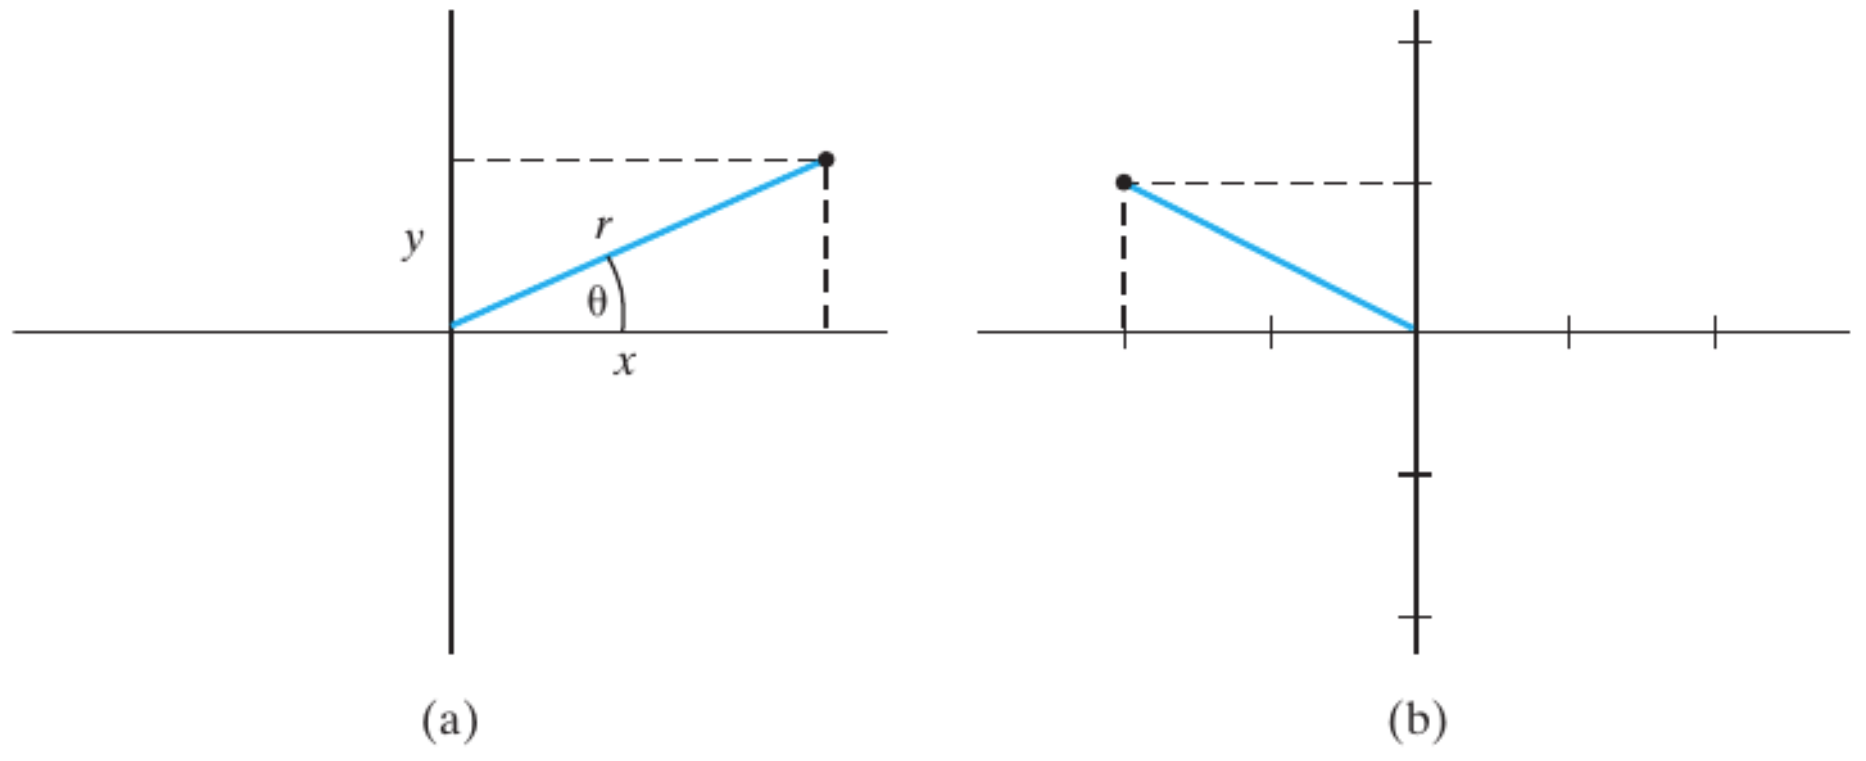
\includegraphics[width=0.78\linewidth]{Figures/fig1_3_complex.png}

    \iqbmicrosep

    {\scriptsize 图1.3：复数在复平面上的表示。(a) $z = x + iy$；(b) $-2 + i$。}
  }
\end{frame}

% ------------------------------------------------------------
% 1.7-2. Euler's Formula and Complex Conjugate
% ------------------------------------------------------------
\begin{frame}{欧拉公式与复共轭}
  \iqbfontsizemode{small}

  \iqblayouttwo{
    \iqbsectiontitle{欧拉公式}
    \begin{iqbitemize}
    \item 复数最重要的公式：
    \end{iqbitemize}
      \[
        \boxed{e^{i\theta} = \cos\theta + i\sin\theta}
      \]
    \begin{iqbitemize}
  \item 指数形式：$\boxed{z = re^{i\theta}}$ 这是复数最简洁、最有用的表示

    \end{iqbitemize}
    \iqbsep

    \iqbsectiontitle{特殊值}
    \begin{iqbitemize}
  \item $\theta = \pi/2$：$e^{i\pi/2} = i$ $\theta = \pi$：$e^{i\pi} = -1$ （\textbf{欧拉恒等式}，Euler's identity）
      \item $\theta = 2\pi$：$e^{i2\pi} = 1$
    \end{iqbitemize}
  }{
    \iqbsectiontitle{复共轭}
    \begin{iqbitemize}
    \item \textbf{复共轭}（complex conjugate）：$z^* = x - iy$
      \item 在复平面上是关于实轴的镜像
      \item 基本性质：
    \end{iqbitemize}
      \[
        z \cdot z^* = (x+iy)(x-iy) = x^2 + y^2 = |z|^2
      \]
      \[
        |z| = \sqrt{z \cdot z^*}
      \]
    \begin{iqbitemize}
      \item 实部和虚部提取：
    \end{iqbitemize}
      \[
        \text{Re}(z) = \dfrac{z + z^*}{2}, \quad \text{Im}(z) = \dfrac{z - z^*}{2i}
      \]
    \begin{iqbitemize}
      \item 运算性质：$(z_1 z_2)^* = z_1^* z_2^*$
    \end{iqbitemize}
  }

  \iqbgreenbox{核心工具}{欧拉公式连接指数函数与三角函数，复共轭在求模和实部虚部时不可或缺}
\end{frame}

% ------------------------------------------------------------
% 1.7-2b. Complex Arithmetic Operations
% ------------------------------------------------------------
\begin{frame}{复数的四则运算}
  \iqbfontsizemode{small}

  \iqblayouttwo{
    \iqbsectiontitle{加减法}
    \begin{iqbitemize}
    \item 直角坐标形式：
    \end{iqbitemize}
      \[
        (x_1 + iy_1) \pm (x_2 + iy_2) = (x_1 \pm x_2) + i(y_1 \pm y_2)
      \]
    \begin{iqbitemize}
      \item 实部和虚部分别相加减
      \item 加法满足交换律、结合律

    \end{iqbitemize}
    \iqbsep

    \iqbsectiontitle{乘法}
    \begin{iqbitemize}
    \item 直角坐标形式：
    \end{iqbitemize}
      \begin{align*}
        (x_1 + iy_1)(x_2 + iy_2) &= (x_1x_2 - y_1y_2) \\
        &\quad + i(x_1y_2 + x_2y_1)
      \end{align*}
    \begin{iqbitemize}
      \item 极坐标形式（\textbf{更简单}）：
    \end{iqbitemize}
      \[
        r_1e^{i\theta_1} \cdot r_2e^{i\theta_2} = r_1r_2 e^{i(\theta_1+\theta_2)}
      \]
    \begin{iqbitemize}
      \item \textbf{模相乘，相位相加}
    \end{iqbitemize}
  }{
    \iqbsectiontitle{除法}
    \begin{iqbitemize}
    \item 直角坐标形式（利用复共轭）：
    \end{iqbitemize}
      \[
        \dfrac{z_1}{z_2} = \dfrac{z_1 z_2^*}{z_2 z_2^*} = \dfrac{z_1 z_2^*}{|z_2|^2}
      \]
    \begin{iqbitemize}
      \item 极坐标形式（\textbf{更简单}）：
    \end{iqbitemize}
      \[
        \dfrac{r_1e^{i\theta_1}}{r_2e^{i\theta_2}} = \dfrac{r_1}{r_2}e^{i(\theta_1-\theta_2)}
      \]
    \begin{iqbitemize}
      \item \textbf{模相除，相位相减}

    \end{iqbitemize}
    \iqbsep

    \iqbsectiontitle{幂运算}
    \begin{iqbitemize}
    \item 极坐标形式：
    \end{iqbitemize}
      \[
        (re^{i\theta})^n = r^n e^{in\theta}
      \]
    \begin{iqbitemize}
      \item 模的$n$次方，相位乘以$n$
      \item 例：$(e^{i\theta})^n = e^{in\theta}$
    \end{iqbitemize}
  }
\end{frame}

% ------------------------------------------------------------
% 1.7-3. Example: Complex Numbers Part 1
% ------------------------------------------------------------
\begin{frame}{例题：复数的模、相位与欧拉恒等式}
  \iqbfontsizemode{small}

  \iqblayouttwo{
    \iqbsectiontitle{问题1：计算复数模和相位}
    \begin{iqbitemize}
    \item 求$z = 3 + 4i$的模和相位
      \item 解：
    \end{iqbitemize}
      \[
        |z| = \sqrt{3^2 + 4^2} = \sqrt{25} = \boxed{5}
      \]
      \[
        \tan\theta = \dfrac{4}{3}, \quad \theta = \arctan(4/3)
      \]
      \[
        \theta \approx \boxed{53.1°}
      \]
    \begin{iqbitemize}
      \item 指数形式：$z = 5e^{i \cdot 53.1°}$

    \end{iqbitemize}
    \iqbsmallsep

    \iqbsectiontitle{几何意义}
    \begin{iqbitemize}
    \item 模$|z| = 5$：复数到原点的距离
      \item 相位$\theta = 53.1°$：与实轴的夹角
      \item 复平面上的点$(3, 4)$对应向量
    \end{iqbitemize}

  \iqbgreenbox{关键公式}{欧拉公式$e^{i\theta} = \cos\theta + i\sin\theta$是复数运算的核心}
  }{
    \iqbsectiontitle{问题2：欧拉恒等式}
    \begin{iqbitemize}
  \item 求证：$e^{i\pi} = -1$
  \item 证明：
    \end{iqbitemize}
      \[
        e^{i\pi} = \cos\pi + i\sin\pi = -1 + i \cdot 0 = \boxed{-1}
      \]
    \begin{iqbitemize}
      \item 移项得到著名的\textbf{欧拉恒等式}：
    \end{iqbitemize}
      \[
        \boxed{e^{i\pi} + 1 = 0}
      \]
    \begin{iqbitemize}
      \item 连接了$e, i, \pi, 1, 0$五个重要常数

    \end{iqbitemize}
    \iqbsep

    \iqbsectiontitle{其他重要值}
    \begin{iqbitemize}
    \item $e^{i\pi/2} = i$
      \item $e^{i2\pi} = 1$
      \item $e^{-i\pi} = -1$
    \end{iqbitemize}
  }
\end{frame}

% ------------------------------------------------------------
% 1.7-3b. Example: nth Roots of Unity
% ------------------------------------------------------------
\begin{frame}{例题：单位根与对称性}
  \iqbfontsizemode{small}

  \iqblayouttwo{
    \iqbsectiontitle{问题：求$n$次单位根}
    \begin{iqbitemize}
    \item 求方程$z^n = 1$的所有复数解
      \item 解：设$z = e^{i\theta}$，则
    \end{iqbitemize}
      \[
        z^n = e^{in\theta} = 1 = e^{i \cdot 2\pi k}
      \]
    \begin{iqbitemize}
      \item 因此：$n\theta = 2\pi k$，即
    \end{iqbitemize}
      \[
        \theta = \dfrac{2\pi k}{n}
      \]
    \begin{iqbitemize}
      \item $k = 0, 1, 2, \ldots, n-1$给出$n$个不同的解

    \end{iqbitemize}
    \iqbsep

    \iqbsectiontitle{通解}
    \begin{iqbitemize}
    \item \textbf{$n$次单位根}：
    \end{iqbitemize}
      \[
        \boxed{z_k = e^{i2\pi k/n}, \quad k = 0, 1, \ldots, n-1}
      \]
    \begin{iqbitemize}
      \item 共有$n$个解
    \end{iqbitemize}
  }{
    \iqbsectiontitle{具体例子：$n=3$}
    \begin{iqbitemize}
    \item $z_0 = e^{i \cdot 0} = 1$
      \item $z_1 = e^{i2\pi/3} = \cos(120°) + i\sin(120°) = -\dfrac{1}{2} + i\dfrac{\sqrt{3}}{2}$
      \item $z_2 = e^{i4\pi/3} = \cos(240°) + i\sin(240°) = -\dfrac{1}{2} - i\dfrac{\sqrt{3}}{2}$

    \end{iqbitemize}
    \iqbsep

    \iqbsectiontitle{几何性质}
    \begin{iqbitemize}
    \item 在复平面上均匀分布在单位圆上
      \item 相邻两根之间的夹角为$\dfrac{2\pi}{n}$
      \item 具有$n$重旋转对称性
      \item 在量子力学中描述对称性和周期性
    \end{iqbitemize}
  }
\end{frame}

% ============================================================
% Part 8: Units (1.8)
% ============================================================
\iqbsectionframe{Units}{国际单位制}

% ------------------------------------------------------------
% 1.8-1. SI Units
% ------------------------------------------------------------
\begin{frame}{SI单位制与库仑定律}
  \iqbfontsizemode{small}

  \iqblayouttwo{
    \iqbsectiontitle{SI基本单位}
    \begin{iqbitemize}
    \item \textbf{国际单位制}（SI，Système International）七个基本单位：
        \subitem{长度：米（m），质量：千克（kg），时间：秒（s）}
          \subitem{电流：安培（A），温度：开尔文（K）}
          \subitem{物质的量：摩尔（mol），发光强度：坎德拉（cd）}
      \item 所有其他单位由基本单位导出

    \end{iqbitemize}
    \iqbtinysep

    \iqbsectiontitle{能量单位}
    \begin{iqbitemize}
    \item SI单位：焦耳（J，Joule）
      \item 常用：kJ/mol（化学）、eV（物理，电子伏特electron-volt）
    \end{iqbitemize}
      \[
        1 \text{ eV} = 1.602 \times 10^{-19} \text{ J}
      \]
  }{
    \iqbsectiontitle{库仑定律（SI表述）}
    \begin{iqbitemize}
    \item 两点电荷$q_1$、$q_2$间的力：
    \end{iqbitemize}
      \[
        \boxed{F = \dfrac{1}{4\pi\varepsilon_0}\dfrac{q_1 q_2}{r^2}}
      \]
    \begin{iqbitemize}
      \item $r$：距离（m），$\varepsilon_0$：真空介电常数
    \end{iqbitemize}
      \[
        \varepsilon_0 = 8.854 \times 10^{-12} \text{ C}^2\text{/(N·m}^2\text{)}
      \]

    \iqbtinysep

    \iqbsectiontitle{静电势能}
    \begin{iqbitemize}
    \item 两点电荷的\textbf{静电势能}（electrostatic potential energy）：
    \end{iqbitemize}
      \[
        V = \dfrac{1}{4\pi\varepsilon_0}\dfrac{q_1 q_2}{r}
      \]
    \begin{iqbitemize}
      \item 量子化学计算电子-核、电子-电子相互作用的基础

    \end{iqbitemize}
  \iqbgreenbox{注意}{本课程使用SI单位制，注意$4\pi\varepsilon_0$因子}
  }
\end{frame}

% ============================================================
% Part 9: Calculus (1.9)
% ============================================================
\iqbsectionframe{Calculus}{微积分公式}

% ------------------------------------------------------------
% 1.9-1. Derivatives
% ------------------------------------------------------------
\begin{frame}{常用导数公式}
  \iqbfontsizemode{small}

  \iqblayouttwo{
    \iqbsectiontitle{基本导数}
    \begin{iqbitemize}
    \item $\dfrac{\mathrm{d}}{\mathrm{d}x}(x^n) = nx^{n-1}$
      \item $\dfrac{\mathrm{d}}{\mathrm{d}x}(e^x) = e^x$
      \item $\dfrac{\mathrm{d}}{\mathrm{d}x}(e^{ax}) = ae^{ax}$
      \item $\dfrac{\mathrm{d}}{\mathrm{d}x}(\ln x) = \dfrac{1}{x}$
      \item $\dfrac{\mathrm{d}}{\mathrm{d}x}(\sin x) = \cos x$
      \item $\dfrac{\mathrm{d}}{\mathrm{d}x}(\cos x) = -\sin x$

    \end{iqbitemize}
    \iqbsmallsep

    \iqbsectiontitle{链式法则}
    \begin{iqbitemize}
    \item $\dfrac{\mathrm{d}}{\mathrm{d}x}f(g(x)) = f'(g(x)) \cdot g'(x)$
      \item 例：$\dfrac{\mathrm{d}}{\mathrm{d}x}e^{-x^2} = e^{-x^2} \cdot (-2x) = -2xe^{-x^2}$
    \end{iqbitemize}
  }{
    \iqbsectiontitle{乘积法则}
    \begin{iqbitemize}
    \item $\dfrac{\mathrm{d}}{\mathrm{d}x}[f(x)g(x)] = f'(x)g(x) + f(x)g'(x)$

    \end{iqbitemize}
    \iqbsmallsep

    \iqbsectiontitle{商法则}
    \begin{iqbitemize}
    \item $\dfrac{\mathrm{d}}{\mathrm{d}x}\left[\dfrac{f(x)}{g(x)}\right] = \dfrac{f'(x)g(x) - f(x)g'(x)}{[g(x)]^2}$

    \end{iqbitemize}
    \iqbsmallsep

    \iqbsectiontitle{偏导数}
    \begin{iqbitemize}
    \item 多变量函数$f(x,y,z)$
  \item 对$x$的偏导数：$\dfrac{\partial f}{\partial x}$ 其他变量$y, z$视为常数
    \end{iqbitemize}
  }
\end{frame}

% ------------------------------------------------------------
% 1.9-2. Integrals
% ------------------------------------------------------------
\begin{frame}{常用积分公式}
  \iqbfontsizemode{small}

  \iqblayouttwo{
    \iqbsectiontitle{基本积分}
    \begin{iqbitemize}
    \item $\int x^n \mathrm{d}x = \dfrac{x^{n+1}}{n+1} + C$ （$n \neq -1$）
      \item $\int \dfrac{1}{x} \mathrm{d}x = \ln|x| + C$
      \item $\int e^x \mathrm{d}x = e^x + C$
      \item $\int e^{ax} \mathrm{d}x = \dfrac{1}{a}e^{ax} + C$
      \item $\int \sin x \mathrm{d}x = -\cos x + C$
      \item $\int \cos x \mathrm{d}x = \sin x + C$

    \end{iqbitemize}
    \iqbsmallsep

    \iqbsectiontitle{重要积分}
    \begin{iqbitemize}
    \item $\int_{-\infty}^{+\infty} e^{-ax^2} \mathrm{d}x = \sqrt{\dfrac{\pi}{a}}$ （$a > 0$）
      \item $\int_0^{\infty} x^n e^{-ax} \mathrm{d}x = \dfrac{n!}{a^{n+1}}$ （$a > 0$, $n$为非负整数）
    \end{iqbitemize}
  }{
    \iqbsectiontitle{分部积分}
    \begin{iqbitemize}
    \item $\int u \, dv = uv - \int v \, du$
      \item 例：$\int x e^x \mathrm{d}x = xe^x - e^x + C$

    \end{iqbitemize}
    \iqbtinysep

    \iqbsectiontitle{换元积分}
    \begin{iqbitemize}
  \item 设$u = g(x)$，$du = g'(x)dx$ $\int f(g(x))g'(x) \mathrm{d}x = \int f(u) du$

    \end{iqbitemize}
    \iqbtinysep

    \iqbsectiontitle{多重积分}
    \begin{iqbitemize}
  \item 三维：$\iiint f(x,y,z) \mathrm{d}x\,\mathrm{d}y\,\mathrm{d}z$ 球坐标体积元：$dV = r^2\sin\theta \, dr\,d\theta\,d\phi$

    \end{iqbitemize}
  \iqbgreenbox{提示}{量子化学中最常用Gaussian积分$\int e^{-ax^2} \mathrm{d}x$}
  }
\end{frame}

% ------------------------------------------------------------
% Acknowledgment
% ------------------------------------------------------------
\begin{frame}[plain]
  \begin{center}
    \vspace*{2cm}
    {\Huge\color{iqbblue}\textbf{谢谢！}}

    \vspace{1cm}

    {\Large Questions?}

    \vspace{2cm}

    {\large 量子化学第一章：薛定谔方程}

    \vspace{0.5cm}

    {\normalsize 参考教材：Levine, \textit{Quantum Chemistry}, 7th Edition}
  \end{center}
\end{frame}

\end{document}
